\documentclass[12pt,a4paper,oneside]{report}
\usepackage[utf8]{vietnam}
\usepackage[vietnamese]{babel}
\usepackage{amsmath,amsxtra,amssymb,latexsym, amscd,amsthm, enumerate}
\usepackage{cases}
\usepackage{graphicx}
\usepackage{caption}
\usepackage{subcaption}
\usepackage{url}
\usepackage[style=numeric,backend=biber]{biblatex}
\usepackage{indentfirst}
\usepackage{ragged2e}

\addto\captionsvietnamese{
	\renewcommand{\bibname}{Tài liệu tham khảo}
}
\setlength{\textwidth}{430pt}

\newtheorem{nx}{Nhận xét}[section]
\newtheorem{dl}{Định lý}[section]
\newtheorem{bd}{Bổ đề} [section]
\newtheorem{dn}{Định nghĩa}[section]
\newtheorem{vd}{Ví dụ} [section]
\newtheorem{md}{Mệnh đề}[section]
\newtheorem{hq}{Hệ quả}[section]
\newtheorem{cy}{Chú ý}[section]
\newtheorem{bt}{Bài tập}
\numberwithin{equation}{section}
\setlength{\textwidth}{15.5cm} %Độ rộng của khối chữ 210-3.5-2=15.5cm

\def\A{\mathcal{A}}
\def\C{\mathbb{C}}
\def\R{\mathbb{R}}
\def\Q{\mathbb{Q}}
\def\Z{\mathbb{Z}}
\def\N{\mathbb{N}}
\def\L{\mathcal{L}}
\def\ln{\ell_p^n}
\def\l1{\ell_1}
\def\lp{\ell_p}
\def\lq{\ell_q}
\def\lo{\ell_{\infty}}
\def\Lp{\mathbf{L_p}}
\def\Lpp{\mathit{L_p}}
\def\Lqq{\mathit{L_q}}
\def\Lo{\mathbf{L_{\infty}}}
\def\Loo{\mathit{L_{\infty}}}
\def\m{\mu}
\def\s{\sigma}
\def\sgn{\text{sign}}
\def\disint{\displaystyle\int}
\def\dissum{\displaystyle\sum}
\def\van{triệt tiêu bên ngoài một tập có độ đo hữu hạn }
\def\hol{bất đẳng thức Hölder }
\def\hkn{hầu khắp nơi}
\def\es{\text{ess sup}}
\def\kgdd{(X,\A,\mu)}
	
\setlength{\voffset}{-20pt}
\setlength{\parsep}{0 pt}
\setlength{\evensidemargin} {-0.94 mm}  %Lề trang phải 2.54cm-0.34cm=2cm
\setlength{\oddsidemargin}{0.96cm}     %Lề trang trái 2.54cm+0.96cm=3.5cm
\setlength{\topmargin}{0.2mm}          %Lề trên 2.54cm-0.04cm=2.5cm
\setlength{\headheight}{0.4cm}             %Chieu cao cua Headerline
\setlength{\headsep}{0.5cm}                %Khoảng cách từ Headerline tới khối chữ trong trang
\setlength{\textheight}{23.7cm}             %Chiều cao của khối chữ trong trang=24.1cm
\setlength{\baselineskip}{20truept}
\renewcommand{\baselinestretch}{1.5} % Dãn dòng
%\renewcommand{\footrulewidth}{0.4cm}
\setlength{\hfuzz}{30pt}

\usepackage{fancybox}

\pagenumbering{roman}\pagestyle{plain}

\allowdisplaybreaks
\renewcommand{\bibname}{Tài liệu tham khảo}
\begin{document}

\thispagestyle{empty}
\thisfancypage{\setlength{\fboxsep}{2pt}\setlength{\fboxrule}{2pt}\doublebox}{} 
\begin{center} %%%%
{\fontsize{14pt}{16}\selectfont BỘ GIÁO DỤC VÀ ĐÀO TẠO}\\
\vskip 0.05cm
{\bf\fontsize{14pt}{16}\selectfont TRƯỜNG ĐẠI HỌC QUY NHƠN}\\
{——————————————}\\
\vskip 2cm
{\bf\fontsize{16pt}{22}\selectfont NGUYỄN NHẬT NAM}

\vskip 3cm
\begin{center}
{\bf\fontsize{22pt}{22}\selectfont Một số phương pháp phân tích ma trận và ứng dụng}

\end{center}

\vskip 2.5cm
{\bf\fontsize{16pt}{22}\selectfont KHÓA LUẬN TỐT NGHIỆP ĐẠI HỌC}\\
\vskip 0.5cm
{\bf\fontsize{16pt}{22}\selectfont Ngành: Toán ứng dụng }\\
\vskip 0.05cm
{\bf\fontsize{16pt}{22}\selectfont Chuyên ngành: Khoa học dữ liệu}\\
\vskip 2.5cm
{\bf\fontsize{16pt}{22}\selectfont Người hướng dẫn: TS.Lâm Thị Thanh Tâm}\\

\vfill
{\bf\fontsize{14pt}{16}\selectfont {Bình Định, 2023}}\\
\end{center}
\newpage
\thispagestyle{empty}

%%%%%%% bìa phụ

\thisfancypage{\setlength{\fboxsep}{2pt}\setlength{\fboxrule}{2pt}\doublebox}{} 
\begin{center} %%%%
{\fontsize{14pt}{16}\selectfont BỘ GIÁO DỤC VÀ ĐÀO TẠO}\\
\vskip 0.05cm
{\bf\fontsize{14pt}{16}\selectfont TRƯỜNG ĐẠI HỌC QUY NHƠN}\\
{——————————————}\\
\end{center}

\vskip 3cm
\begin{center}
{\bf\fontsize{22pt}{22}\selectfont Một số phương pháp phân tích ma trận và ứng dụng}



\vskip 3.5cm
{\bf\fontsize{16pt}{22}\selectfont KHÓA LUẬN TỐT NGHIỆP ĐẠI HỌC}\\
\vskip 0.5cm
{\bf\fontsize{16pt}{22}\selectfont Ngành: Toán ứng dụng}\\
\vskip 0.05cm
{\bf\fontsize{16pt}{22}\selectfont Chuyên ngành: Khoa học dữ liệu}\\
\vskip 2.5cm
\end{center}
\begin{flushleft}
{\bf\fontsize{16pt}{22}\selectfont Sinh viên thực hiện:  NGUYỄN NHẬT NAM}\\
\vskip 0.05cm
{\fontsize{16pt}{22}\selectfont Mã số SV: 4251140002}\\
\vskip 0.05cm
{\fontsize{16pt}{22}\selectfont Lớp, Khóa: Toán ứng dụng K42}\\
\vskip 2cm
{\bf\fontsize{16pt}{22}\selectfont Người hướng dẫn: TS.Lâm Thị Thanh Tâm}\\
\end{flushleft}


\vfill
\begin{center}
	{\bf\fontsize{14pt}{16pt}\selectfont Bình Định, 2023}
\end{center}
%\newpage
%\thispagestyle{empty}
%\begin{center}
%	BỘ GIÁO DỤC VÀ ĐÀO TẠO\\
%	\textbf{TRƯỜNG ĐẠI HỌC QUY NHƠN}\\
%	{——————————————}
%
%\end{center}
%\vskip 2.5cm
%\begin{center}
%	\LARGE{\textbf{MỘT SỐ VẤN ĐỀ VỀ KHÔNG GIAN LEBESGUE}}
%	
%	\vskip 0.5cm
%\end{center}
%\vskip 2.5cm
%\begin{center}
%	\textbf{LUẬN VĂN TỐT NGHIỆP ĐẠI HỌC}\\
%	\vskip 0.5cm
%	\textbf{Ngành: Sư phạm Toán}\\
%	\vskip 0.5cm
%	\textbf{Chuyên ngành: Giải tích}
%\end{center}
%\vskip 2cm
%\begin{flushleft}
%	\textbf{Sinh viên thực hiện: Nguyễn Chí Trọng}\\
%	Mã số SV: 3951010051\\
%	Lớp, Khóa: Sư phạm Toán K39
%\end{flushleft}
%\vskip 1.5cm
%
%\begin{center}
%	\textbf{Người hướng dẫn: PGS.TS. LƯƠNG ĐĂNG KỲ}
%\end{center}
%\vskip 1.5cm
%\vfill 
%\begin{center}
%	\textbf{	Bình Định - 2020}
%\end{center}
%


\newpage
\chapter*{Lời cảm ơn}
\pagenumbering{arabic}            % Danh lai trang
\pagenumbering{roman}
\addcontentsline{toc}{chapter}{Lời cảm ơn}
\begin{justify}
Trước khi đi vào nội dung của khóa luận, em xin bày tỏ lòng biết ơn chân thành tới toàn thể giáo viên của Trường Đại học Quy Nhơn nói chung và của Khoa Toán-Thống kê nói riêng vì đã tận tâm dạy bảo em trong suốt quá trình em theo học tại trường, và đặc biệt là sự định hướng dẫn dắt của TS.Lâm Thị Thanh Tâm đối với đề tài khóa luận này.

Nhân dịp này em cũng xin được gửi những lời cảm ơn đến những người bạn, đặc biệt là những người thân trong gia đình đã luôn giúp đỡ em hết mình, luôn động viên, cổ vũ tinh thần và tạo điều kiện thuận lợi giúp em có thể hoàn thành được khoá luận tốt nghiệp này.

Trong quá trình viết khóa luận này mặc dù đã được chỉnh sửa nhiều lần nhưng không thể tránh khỏi việc thiếu sót. Em xin chân thành cảm ơn nếu nhận được sự góp ý từ các quý thầy cô, anh chị và bạn bè để có thể chỉnh sửa luận văn được tốt hơn.
\end{justify}
\vskip 0.5cm
\begin{flushright}
Quy Nhơn, ngày ... tháng ... năm 2023\qquad\\
Sinh viên thực hiện\qquad\qquad\qquad\qquad\\

\vskip 2.5cm
\textbf{  Nguyễn Nhật Nam}\qquad\quad\quad\quad\qquad\\
\end{flushright}

%%% ---------- MỤC LỤC -------- %%%
\tableofcontents
%\chapter*{Một số ký hiệu}
%\addcontentsline{toc}{chapter}{Một số ký hiệu}

%\begin{tabular}{l l}
%	$\mathbb N$&Tập các số tự nhiên,\\ 
%	$\mathbb Z$&Tập các số nguyên,\\
%	$\mathbb Q$&Tập các số hữu tỉ,\\
%	$\mathbb R$&Tập các số thực,\\
%	$\mathbb C$&Tập các số phức,\\
%	$\overline{\mathbb{R}}$& Tập số thực mở rộng $\{-\infty\}\cup\mathbb R\cup\{\infty\},$\\
%	$\mathbb R^n$&Không gian vectơ thực $n$-chiều,\\ 
%	$\chi_A$&Hàm đặc trưng của tập $A$,\\
%	$\bigsqcup\limits_{i=1}^n A_i$&hợp rời rạc các tập $A_1,A_2,\ldots,A_n$.	
%\end{tabular}
\chapter*{Lời mở đầu}
\addcontentsline{toc}{chapter}{Lời mở đầu}

\begin{justify}   
Trong thời đại công nghệ thông tin phát triển mạnh mẽ ngày nay, việc thu thập và xử lý dữ liệu ngày càng trở nên quan trọng và cần thiết. Các phương pháp phân tích dữ liệu như phân rã giá trị kì dị (SVD) và phân tích thành phần chính (PCA) đóng vai trò quan trọng trong việc giải quyết các vấn đề liên quan đến dữ liệu lớn và đa chiều. Những phương pháp này không chỉ giúp giảm kích thước dữ liệu mà còn giúp khai thác thông tin hữu ích từ dữ liệu gốc. SVD và PCA đã và đang được ứng dụng rộng rãi trong nhiều lĩnh vực khoa học và kỹ thuật, chẳng hạn như xử lý hình ảnh, phân tích dữ liệu, nhận dạng mẫu, thống kê,...

Trong khóa luận này, chúng tôi tập trung nghiên cứu về các phương pháp phân tích dữ liệu như phân rã giá trị kì dị (SVD) và phân tích thành phần chính (PCA), cũng như một số ứng dụng của chúng trong bài toán thực tế. Mục tiêu chính của khóa luận là tìm hiểu về các tính chất cơ bản, cách tính và ứng dụng của SVD và PCA trong việc giải quyết các vấn đề liên quan đến dữ liệu.

Đối tượng nghiên cứu trong khóa luận này là phương pháp phân rã giá trị kì dị (SVD) và phân tích thành phần chính (PCA). Ngoài lời cảm ơn, mục lục, lời mở đầu và một số ký hiệu, luận văn được chia làm bốn chương chính:

Chương 1: Kiến thức cơ bản. Trong chương này, chúng tôi trình bày một số kiến thức cơ sở về đại số tuyến tính, giải tích và thống kê, nhằm chuẩn bị cho việc tìm hiểu về SVD và PCA.

Chương 2: Phân rã giá trị kì dị (SVD). Trong chương này, chúng tôi giới thiệu về SVD và các tính chất của ma trận liên quan đến SVD.

Chương 3: Phân tích thành phần chính (PCA). Trong chương này, chúng tôi giới thiệu về PCA, cách tính PCA và mối quan hệ giữa PCA và SVD.

Chương 4: Ứng dụng của SVD và PCA trong bài toán thực tế. Chương này sẽ trình bày một số ví dụ cụ thể về việc áp dụng SVD và PCA trong các bài toán thực tế như xử lý hình ảnh, nhận dạng mẫu, phân tích dữ liệu và thống kê.

Khóa luận tốt nghiệp này được hoàn thành dưới sự hướng dẫn của TS.lâm Thị Thanh Tâm. Nhân dịp này, tôi xin bày tỏ lòng biết ơn sâu sắc đến thầy/cô hướng dẫn, đã không chỉ hỗ trợ tôi trong việc nghiên cứu khoa học mà còn tận tình giúp đỡ và tạo mọi điều kiện thuận lợi cho tôi trong suốt quá trình làm đề tài. Tôi cũng xin chân thành cảm ơn tập thể lớp Toán Ứng Dụng K42, Khoa Toán và Thống kê Trường Đại học Quy Nhơn đã giúp đỡ và tạo mọi điều kiện thuận lợi cho tôi hoàn thành khóa học cùng với luận văn này.

Cuối cùng, tôi xin chân thành cảm ơn gia đình, bạn bè, những người thân yêu đã luôn quan tâm, giúp đỡ và ủng hộ tôi trong suốt quá trình học tập và thực hiện khóa luận này. Dù đã cố gắng hết sức, nhưng do thời gian và năng lực có hạn, khóa luận không tránh khỏi những thiếu sót và hạn chế. Rất mong nhận được sự góp ý và chỉ bảo của quý thầy cô, quý bạn đồng nghiệp để khóa luận tốt nghiệp này được hoàn thiện hơn. Tôi xin chân thành cảm ơn.
\end{justify}
  \chapter*{\centerline{Một số ký hiệu}}
\addcontentsline{toc}{chapter}{Một số ký hiệu}
\begin{tabular}{l l}
	$\mathbb N$&tập các số tự nhiên\\
	$\mathbb Z$&tập các số nguyên\\
	$ \mathbb Q $& tập các số hữu tỷ\\
	$\mathbb R$&tập các số thực\\
	$\mathbb C$&tập các số phức\\
	$ \overline{\R} $&tập các số thực mở rộng\\
	$\mathbb R^n$&không gian vectơ thực $n$-chiều\\ 
	$\mathbb K$&tập $\R$ hoặc $\C$\\
$\mathcal{P}(X)$&tập tất cả các tập con của $X$\\

%	$\gt{\rst}$& tập số thực mở rộng $\{-\vc\}\cup\rst\cup\{\vc\},$\\



%	$\sigma(\uon{C})$&$\sigma$-đại số sinh bởi  $\uon{C}$,\\ 
%	$\uon{M}_L$&$\sigma$-đại số các tập Lebesgue đo được trên $\rst$,\\
%	$\uon{M}_L^n$&$\sigma$-đại số các tập Lebesgue đo được trên $\rst^n$,\\
%	$\uon{C}_c(\rst)$&không gian các hàm liên tục có giá compact,\\ 

%	$\mu_L$&độ đo Lebesgue trên $\rst$,\\
%	$\mu_L^n$&độ đo Lebesgue trên $\rst^n$,\\
%	$(\rst,\uon{M}_L,\mu_L)$&không gian độ đo Lebesgue trên $\rst$,\\
%	$(\rst^n,\uon{M}_L^n,\mu_L^n)$&không gian độ đo Lebesgue trên $\rst^n$,\\
$ \sgn $&hàm dấu\\
$A\bigtriangleup B$&hiệu đối xứng của hai tập $A$ và $B$\\
$\bigsqcup_{i=1}^n A_i$&hợp rời nhau các tập $A_1,\ldots,A_n$\\
$f_n\uparrow$&dãy $f_n$ đơn điệu tăng\\
$f_n\downarrow$&dãy $f_n$ đơn điệu giảm\\
$f_n\nearrow f$&dãy $f_n$ đơn điệu tăng và hội tụ đến $f$\\
$f_n\rightrightarrows f$&dãy $f_n$ hội tụ đều đến $f$\\	
	%$f^+,\ f^-$&phần dương, phần âm của hàm $f$,\\
$\L$&$\sigma$-đại số Lebesgue các tập con của $\R$\\
$m$&độ đo Lebesgue\\
$\sharp$&độ đo đếm
	
\end{tabular}
\chapter{Một số kiến thức chuẩn bị}
\pagenumbering{arabic}            % Danh lai trang
\section{Ma trận}.
\begin{dn}\rm                    %ĐN sigma đại số
 Ma trận cỡ $m \times n$ là một bảng gồm $m n$ số thực được sắp xếp thành $m$ dòng và $n$ cột. Ma trận thường được kí hiệu như sau\\
 $$
 \mathbf{A}=\left[\begin{array}{ccccccc}
 	a_{11} & a_{12} & a_{13} & \cdots & \cdots & \cdots & a_{1 n} \\
 	a_{21} & a_{22} & a_{23} & \cdots & \cdots & \cdots & a_{2 n} \\
 	\vdots & \vdots & \vdots & \cdots & \cdots & \cdots & \vdots \\
 	a_{m 1} & a_{m 2} & a_{13} & \cdots & \cdots & \cdots & a_{m n}
 \end{array}\right],
 $$
 
 hoặc
 
 $$
 \mathbf{A}=\left(\begin{array}{ccccccc}
 	a_{11} & a_{12} & a_{13} & \cdots & \cdots & \cdots & a_{1 n} \\
 	a_{21} & a_{22} & a_{23} & \cdots & \cdots & \cdots & a_{2 n} \\
 	\vdots & \vdots & \vdots & \cdots & \cdots & \cdots & \vdots \\
 	a_{m 1} & a_{m 2} & a_{13} & \cdots & \cdots & \cdots & a_{m n}
 \end{array}\right),
 $$
 
 hoặc $\mathbf{A}=\left(a_{i j}\right)_{m \times n}$, trong đó $a_{i j}$ là phần tử của ma trận nằm trên dòng $i$, cột $j$, với $i=1,2, \ldots, m$ và $j=1,2, \ldots, n$.
 
 Khi $m=n$, ta gọi ma trận cỡ $m \times m$ là ma trận vuông cấp $m$. Các phần tử $a_{11}$, $a_{22}, \ldots, a_{m m}$ nằm trên một đường thẳng được gọi đường chéo chính của ma trận.
\end{dn}
	
%\end{dn}
\begin{dn}\rm
	Ma trận đơn vị cấp $n$ là ma trận vuông cấp $n$ có mọi phần tử nằm trên đường chéo chính bằng 1, các phần tử khác bằng 0. Ta ký hiệu ma trận đơn vị cấp $n$ bởi $\mathbf{I}_{n}$ và nó có dạng như sau
$$
\mathbf{I}_{n}=\left[\begin{array}{cccc}
	1 & 0 & \cdots & 0 \\
	0 & 1 & \cdots & 0 \\
	\vdots & \vdots & \ddots & \vdots \\
	0 & 0 & \ldots & 1
\end{array}\right]
$$
Trong trường hợp không cần chú ý đến cấp của ma trận, ta ký hiệu ma trận đơn vị bởi $\mathbf{I}$ .
\end{dn}
\begin{dn}\rm                     
Ma trận đường chéo là ma trận vuông có các phần tử nằm trên đường chéo chính khác 0, các phần tử nằm ngoài đường chéo chính bằng 0. Ma trận đường chéo có dạng như sau
$$
\mathbf{D}=\left[\begin{array}{cccc}
	a_{11} & 0 & \ldots & 0 \\
	0 & a_{22} & \cdots & 0 \\
	\vdots & \vdots & \ddots & \vdots \\
	0 & 0 & \ldots & a_{m m}
\end{array}\right]
$$
\indent Ma trận chỉ có một dòng được gọi là vector dòng. Ma trận chỉ có một cột được gọi là vector cột.
\end{dn}
\begin{dn}\rm 
	Ma trận vuông A cấp $n$ được gọi là ma trận khả nghịch nếu tồn tại một ma trận $\mathbf{A}^{\prime}$ vuông cấp $n$ thỏa mãn $\mathbf{A} \mathbf{A}^{\prime}=\mathbf{A}^{\prime} \mathbf{A}=\mathbf{I}_{n}$. Ma trận $\mathbf{A}$ được gọi là ma trận nghịch đảo của ma trận $\mathbf{A}$, và được ký hiệu là $\mathbf{A}^{-1}$
\end{dn}
\begin{dn}\rm 
	Cho ma trận $\mathbf{A}=\left(a_{i j}\right)_{m \times n}$. Ma trận chuyển vị của $\mathbf{A}$, ký hiệu là $\mathbf{A}^{T}$, có dạng $\mathbf{A}^{T}=\left(a_{j i}\right)_{n \times m}$.
	
	Ma trận vuông $\mathbf{A}$ được gọi là ma trận đối xứng nếu $\mathbf{A}^{T}=\mathbf{A}$, và được gọi là ma trận phản đối xứng nếu $\mathbf{A}^{T}=-\mathbf{A}$.
\end{dn}
\begin{dn}\rm 
	Ma trận vuông $\mathbf{A}$ được gọi là ma trận trực giao nếu $\mathbf{A}^{T} \mathbf{A}=$ $\mathbf{A A}^{T}=\mathbf{I}$
\end{dn}	
	Nhận xét:
	\begin{itemize}
	
	\item[(i)] Ma trận $\mathbf{A}=\left[a_{i j}\right]_{n \times n}$ là ma trận trực giao khi và chỉ khi $$\sum_{k=1}^{n} a_{i k} a_{j k}=\delta_{i j}$$ với $\delta_{i j}$ là kí hiệu Kronecker. 
	
	\item[(ii)] Ma trận trực giao $\mathbf{A}$ là khả nghịch và $\mathbf{A}^{T}=\mathbf{A}^{-1}$.
	
	\item[(iii)]  Ma trận $\mathbf{A}$ trực giao khi và chỉ khi các vector cột và các vector hàng của $\mathbf{A}$ tạo thành các hệ trực chuẩn.
	\end{itemize}
\begin{dn}\rm 
	Cho $\mathbf{A}$ là một ma trận vuông cấp $n$. Định thức của ma trận $\mathbf{A}$, ký hiệu là $\operatorname{det}(\mathbf{A})$ hay $|\mathbf{A}|$ là một giá trị được xác định bằng công thức
	
	$$
	\operatorname{det}(\mathbf{A})=a_{11} \mathbf{A}_{11}+a_{12} \mathbf{A}_{12}+\cdots+a_{1 n} \mathbf{A}_{1 n}
	$$
	trong đó $\mathbf{A}_{i k}=(-1)^{i+k} \operatorname{det}\left(\mathbf{M}_{i k}\right)$, với $\mathbf{M}_{i k}$ là ma trận vuông cấp $n-1$ nhận được từ ma trận $\mathbf{A}$ bằng cách bỏ đi dòng thứ $i$ và cột thứ $k$. Đại lượng $\mathbf{A}_{i k}$ được gọi là phần bù đại số của $a_{i k}$.
	
	Nhận xét:
	
	- Định thức cấp một: Nếu $\mathbf{A}=\left(a_{11}\right)$ thì $\operatorname{det}(\mathbf{A})=a_{11}$.
	
	- Định thức cấp hai: Nếu $\mathbf{A}=\left[\begin{array}{ll}a & b \\ c & d\end{array}\right]$ thì $\operatorname{det}(\mathbf{A})=a d-b c$.
\end{dn}
\begin{dn}\rm 
	Cho $\mathbf{A}$ là ma trận cỡ $m \times n$ bất kì và $s$ là số nguyên thỏa $1 \leqslant s \leqslant \min (m, n)$. Khi đó, các phần tử nằm trên giao của $s$ dòng và $s$ cột của ma trận $\mathbf{A}$ sẽ lập nên các ma trận vuông cấp $s$, ta gọi đó chính là các ma trận con cấp $s$ của $\mathbf{A}$.
	
	Định thức của các ma trận này được gọi là định thức con cấp $s$ của ma trận $\mathbf{A}$.
\end{dn}
\begin{dn}\rm 
	 Định thức con cấp cao nhất, khác 0 của ma trận $\mathbf{A}$ được gọi là định thức con cơ sở của ma trận $\mathbf{A}$. Một ma trận $\mathbf{A}$ có thể có nhiều định thức con cơ sở cùng cấp.
	
	Hạng của ma trận $\mathbf{A}$ là cấp của định thức con cơ sở. Ký hiệu hạng của ma trận $\mathbf{A}$ là $\operatorname{rank}(\mathbf{A})$.
	
	Nhận xét: Cho $\mathbf{A}$ là ma trận cấp $m \times n, \mathbf{B}$ là ma trận cấp $n \times l$.
	\begin{itemize}
	 \item[(i)] Nếu $\operatorname{rank}(\mathbf{B})=n$ thì $\operatorname{rank}(\mathbf{A} \cdot \mathbf{B})=\operatorname{rank}(\mathbf{A})$.
	
	 \item[(ii)] Nếu $\operatorname{rank}(\mathbf{A})=n$ thì $\operatorname{rank}(\mathbf{A} . \mathbf{B})=\operatorname{rank}(\mathbf{B})$.
	\end{itemize}
\end{dn}
\begin{dn}\rm 
	Vết của ma trận vuông $\mathbf{A}$ cấp $n$ được xác định bằng tổng các phần tử trên đường chéo chính của ma trận $\mathbf{A}$, và được ký hiệu là $\operatorname{Tr}(\mathrm{A})$.
\end{dn}

\section{Vector riêng- Giá trị riêng}
\begin{dn}\rm
 Cho $\mathbf{A}$ là ma trận vuông cấp $n$. Khi đó đa thức bậc $n$ của biến $\lambda$ được xác định như sau
 $$
 P_{\mathbf{A}}(\lambda)=\operatorname{det}(\mathbf{A}-\lambda \mathbf{I})=\left|\begin{array}{cccc}
 	a_{11}-\lambda & a_{12} & \ldots & a_{1 n} \\
 	a_{21} & a_{22}-\lambda & \ldots & a_{2 n} \\
 	\vdots & \vdots & \ddots & \vdots \\
 	a_{n 1} & a_{n 2} & \ldots & a_{n n}-\lambda
 \end{array}\right|
 $$
được gọi là đa thức đặc trưng của ma trận $\mathbf{A}$. Các nghiệm của đa thức $P_{\mathbf{A}}(\lambda)$ được gọi là các giá trị riêng của ma trận $\mathbf{A}$.\\
Vector $\mathbf{u} \in \mathbb{R}^{n}$ được gọi là vector riêng ứng với giá trị riêng $\lambda$ của ma trận $\mathbf{A}$ nếu thỏa $\mathbf{A u}=\lambda \mathbf{u}$.
\end{dn}
Nhận xét:
\begin{itemize}
 \item[(i)] Nếu $\lambda$ là một giá trị riêng của $\mathbf{A}$ thì $\operatorname{det}(\mathbf{A}-\lambda \mathbf{I})=0$. Khi đó hệ phương trình thuần nhất 
 $$
 (\mathbf{A}-\lambda \mathbf{I})\left[\begin{array}{c}
 	x_{1} \\
 	\vdots \\
 	x_{n}
 \end{array}\right]=0
 $$
 
 có vô số nghiệm.
 
 \item[(ii)] Mỗi giá trị riêng có thể có nhiều vector riêng.
 
 \item[(iii)] Mỗi vector riêng chỉ ứng với một giá trị riêng duy nhất.
 
 \item[(iv)] Nếu $\lambda=0$ là một giá trị riêng của ma trận $\mathbf{A}$ thì $\mathbf{A}$ không khả nghịch. Ngược lại, nếu mọi giá trị riêng của $\mathbf{A}$ đều khác 0 thì ma trận $\mathbf{A}$ khả nghịch. 
\end{itemize}

\section{Định lí phổ của ma trận đối xứng}
\begin{dn} \label{dlpho}
Cho $\mathbf{A}$ là ma trận đối xứng cấp $n$. Khi đó:
\begin{itemize}
\item[(i)] Với mỗi giá trị riêng thực $\lambda$ của $\mathbf{A}$, tồn tại một vector riêng tương ứng $\mathbf{u} \in \mathbb{R}^{n}$ sao cho $\mathbf{A u}=\lambda \mathbf{u}$.

\item[(ii)] Tồn tại ma trận dường chéo $\mathbf{D}$ cấp $n$ và ma trận trực giao $\mathbf{U}$ cấp $n$ sao cho $\mathbf{A}=\mathbf{U D U}^{T}$, trong đó các phần tử nằm trên đường chéo chính của $\mathbf{D}$ là các giá trị riêng của $\mathbf{A}$, và các vector cột của $\mathbf{U}$ là các vetor riêng của $\mathbf{A}$ tương ứng với các giá trị riêng đó. Tức là, nếu

$$
\mathbf{D}=\operatorname{diag}\left(\lambda_{1}, \lambda_{2}, \ldots, \lambda_{n}\right)
$$

và

$$
\mathbf{U}=\left[\begin{array}{lllllll}
	\mathbf{u}^{(1)} & \mid & \mathbf{u}^{(2)} & \ldots & \ldots & \mathbf{u}^{(n)}
\end{array}\right]
$$

thì $\mathbf{A} \mathbf{u}^{(i)}=\lambda_{i} \cdot \mathbf{u}^{(i)}, \quad i=1,2, \ldots, n$.
\end{itemize}
\end{dn}
%\textbf{Chứng minh}.
\begin{proof}
 Ta sẽ chứng minh định lí này bằng phương pháp quy nạp toán học. Trường hợp $n=1$, kết quả trên đúng. Giả sử kết quả trên đúng với mọi ma trận có cấp nhỏ hơn hoặc bằng $n-1$, ta sẽ chứng minh kết quả trên đúng trong trường hợp ma trận $\mathbf{A}$ là ma trận đối xứng cấp $n$.
	
	Xét hàm số $p(t)=\operatorname{det}(t \mathbf{I}-\mathbf{A})$. Ta có $p(t)$ là một đa thức bậc $n$ và được gọi là đa thức đặc trưng của ma trận $\mathbf{A}$. Theo Định lí cơ bản của đại số, đa thức $p(t)$ sẽ có $n$ nghiệm là $\lambda_{1}, \lambda_{2}, \ldots, \lambda n$, và ta gọi chúng là các giá trị riêng của ma trận $\mathbf{A}$.
	
	Giả sử $\lambda$ là một giá trị riêng của ma trận $\mathbf{A}$, ta có $\operatorname{det}(\lambda \mathbf{I}-\mathbf{A})=0$, tức ma trận $(\lambda \mathbf{I}-\mathbf{A})$ không khả nghịch. Điều này có nghĩa là, tồn tại một vector thực, khác không $\mathbf{u}$ sao cho $\mathbf{A} \mathbf{u}=\lambda \mathbf{u}$. Ta có thể chuẩn hóa vector $\mathbf{u}$ sao cho $\mathbf{u}^{T} \mathbf{u}=1$. Khi đó, $\lambda=\mathbf{u}^{T} \mathbf{A u}$ là số thực.
	
	Với $\lambda_{1}$ là một giá trị riêng của $\mathbf{A}$ và $\mathbf{u}_{1}$ là một vector riêng tương ứng. Sử dụng phép trực giao hóa Gramm-Schmidt, ta có thể tìm được ma trận $\mathbf{V}_{1}$ cấp $n \times(n-1)$ sao cho $\left[\mathbf{u}_{1} \mathbf{V}_{1}\right]$ là một ma trận trực giao. Ta có $\mathbf{V}_{1}^{T} \mathbf{A} \mathbf{V}_{1}$ là ma trận đối xứng cấp $n-1$. Khi đó theo giả thiết quy nạp, ta có thể viết $\mathbf{V}_{1}^{T} \mathbf{A} \mathbf{V}_{1}=\mathbf{Q}_{1} \mathbf{D}_{1} \mathbf{Q}_{1}^{T}$, trong đó $\mathbf{D}_{1}=\operatorname{diag}\left(\lambda_{2}, \lambda_{3}, \ldots, \lambda_{n}\right)$ là ma trận đường chéo với các phần tử nằm trên đường chéo chính là $n-1$ giá trị riêng của $\mathbf{A}$ và $\mathbf{Q}_{1}$ là ma trận trực giao cấp $(n-1)$ gồm $(n-1)$ vector riêng của $\mathbf{V}_{1}^{T} \mathbf{A} \mathbf{V}_{1}$ tương ứng.
	
	Ta định nghĩa ma trận $\mathbf{U}_{1}$ cấp $n \times(n-1)$ bởi $\mathbf{U}_{1}=\mathbf{V}_{1} \mathbf{Q}_{1}$. Khi đó $\mathbf{U}=\left[\mathbf{u}_{1}, \mathbf{U}_{1}\right]$ là ma trận trực giao. Ta có
	
	$$
	\mathbf{U}^{T} \mathbf{A} \mathbf{U}=\left(\begin{array}{c}
		\mathbf{u}_{1}^{T} \\
		\mathbf{U}_{1}^{T}
	\end{array}\right) \mathbf{A}\left(\mathbf{u}_{1}-\mathbf{U}_{1}\right)=\left(\begin{array}{cc}
		\mathbf{u}_{1}^{T} \mathbf{A} \mathbf{u}_{1} & \mathbf{u}_{1}^{T} \mathbf{A} \mathbf{U}_{1} \\
		\mathbf{U}_{1}^{T} \mathbf{A} \mathbf{u}_{1} & \mathbf{U}_{1}^{T} \mathbf{A} \mathbf{U}_{1}
	\end{array}\right)=\left(\begin{array}{cc}
		\lambda_{1} & 0 \\
		0 & \mathbf{D}_{1}
	\end{array}\right)=\mathbf{D} .
	$$
	Điều này chứng tỏ $\mathbf{A}=\mathbf{U D U}^{T}$, với $\mathbf{U}$ là ma trận trực giao cấp $n$ và $\mathbf{D}=$ $\operatorname{diag}\left(\lambda_{1}, \lambda_{2}, \ldots, \lambda_{n}\right).$\\
	Đây được gọi là phân tích giá trị riêng của ma trận $\mathbf{A}$ (Eigen value decomposition, EVD). 
\end{proof}
\section{Xác xuất thống kê}
\subsection{Kỳ vọng}
\label{sub:expectaion_covariance}
\index{kỳ vọng -- expectation}
\textit{Kỳ vọng} (expectation) của một biến ngẫu nhiên $\mathbf{x}$ được định nghĩa bởi:
	\begin{eqnarray}
		\label{eqn:30_21}
		\text{E}[\mathbf{x}] = \sum_ \mathbf{x} \mathbf{x} p(\mathbf{x})  & \text{nếu}~\mathbf{ x} ~ \text{là rời rạc.} \quad
		\\
		\label{eqn:30_22}
		\text{E}[\mathbf{x}] = \int \mathbf{x} p(\mathbf{x}) dx  & \text{nếu}~ \mathbf{x} ~ \text{là liên tục.}
	\end{eqnarray}
	% \end{equation}
Giả sử $f(.)$ là một hàm số trả về một số với mỗi giá trị $\mathbf{x^*}$ của biến ngẫu
nhiên $\mathbf{x}$. Khi đó, nếu $\mathbf{x}$ là biến ngẫu nhiên rời rạc, ta có
\begin{equation}
	\label{eqn:30_23}
	\text{E}[f(\mathbf{x})] = \sum_\mathbf{x} f(\mathbf{x}) p(\mathbf{x}).
\end{equation}
Công thức cho biến ngẫu nhiên liên tục cũng được viết tương tự.

Với xác suất đồng thời, kỳ vọng của một hàm cũng được xác định tương tự:
\begin{equation}
	\label{eqn:30_24}
	\text{E}[f(x, y)] = \sum_{\mathbf{x,y}} f(\mathbf{x, y}) p(\mathbf{x, y}) dx dy.
\end{equation}
Có ba tính chất cần nhớ về kỳ vọng:
\begin{enumerate}
	\item Kỳ vọng của một hằng số theo một biến ngẫu nhiên $\mathbf{x}$ bất kỳ bằng chính hằng số đó:
	\begin{equation}
		\label{eqn:30_25}
		\text{E}[\alpha] = \alpha.
	\end{equation}
	\item Kỳ vọng có tính chất tuyến tính:
	\begin{eqnarray}
		\label{eqn:30_26}
		\text{E}[\alpha \mathbf{x}] & = & \alpha \text{E}[\mathbf{x}],  \\
		\label{eqn:30_27}
		\text{E}[f(\mathbf{x}) + g(\mathbf{x})] & = & \text{E}[f(\mathbf{x})] + \text{E}[g(\mathbf{x})].
	\end{eqnarray}
	\item Kỳ vọng của tích hai biến ngẫu nhiên độc lập bằng tích kỳ vọng của chúng:
	\begin{equation}
		\label{eqn:30_28}
		\text{E}[f(\mathbf{x}) g(\mathbf{y})] = \text{E}[f(\mathbf{x})] \text{E}[g(\mathbf{y})].
	\end{equation}
	
\end{enumerate}


% \subsection{Kỳ vọng và ma trận hiệp phương sai}

Khái niệm kỳ vọng thường đi kèm với khái niệm \textit{phương
	sai} (variance) trong không gian một chiều và \textit{ma trận hiệp
	phương sai} (covariance matrix) trong không gian nhiều chiều. 

\subsection{Phương sai} % (fold)

% \subsubsection{Với dữ liệu một chiều}
\index{phương sai -- variance}
\index{do@độ lệch chuẩn -- standard deviation}
Cho $N$ giá trị $\mathbf{x}_1, \mathbf{x}_2, \dots, \mathbf{x}_N$. {Kỳ vọng} và {phương sai}
của bộ dữ liệu này được tính theo công thức
\begin{eqnarray} 
	\bar{\mathbf{x}} &=& \frac{1}{N}\sum_{n=1}^N \mathbf{x}_n = \frac{1}{N}\mathbf{x1},\\\ 
	\sigma^2 &=& \frac{1}{N} \sum_{n=1}^N (\mathbf{x}_n - \bar{\mathbf{x}})^2,
\end{eqnarray} 
$\text { với } \mathbf{x}=\left[x_1, x_2, \ldots, x_N\right] \text {, và } \mathbf{1} \in \mathbb{R}^N$là
vector cột chứa toàn phần tử 1. Kỳ vọng đơn giản là trung bình cộng của toàn bộ
các giá trị. Phương sai là trung bình cộng của bình phương khoảng cách từ mỗi
điểm tới kỳ vọng. Phương sai càng nhỏ, các điểm dữ liệu càng gần với kỳ vọng,
tức các điểm dữ liệu càng giống nhau. Phương sai càng lớn, dữ liệu càng có tính
phân tán. Ví dụ về kỳ vọng và phương sai của dữ liệu một chiều có thể được thấy
trong Hình~\ref{fig:27_2a}. 

Căn bậc hai của phương sai, $\sigma$ còn được gọi là \textit{độ lệch chuẩn} (standard deviation) của
dữ liệu.


%%%%%%% Three subfigures with bottom caption%%%%%%%%%%%%%%
\begin{figure}[t]
	\begin{subfigure}{0.325\textwidth}
		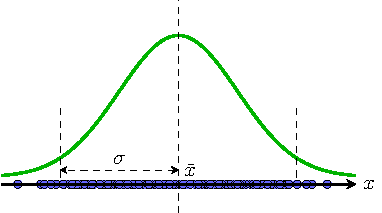
\includegraphics[width=0.99\linewidth]{var_1d.pdf}
		\caption{}
		\label{fig:27_2a}
	\end{subfigure}
	\begin{subfigure}{0.325\textwidth}
		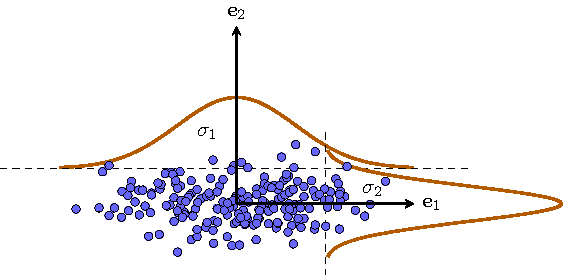
\includegraphics[width=0.99\linewidth]{pca_diagvar.pdf}
		\caption{}
		\label{fig:27_2b}
	\end{subfigure}
	\begin{subfigure}{0.325\textwidth}
		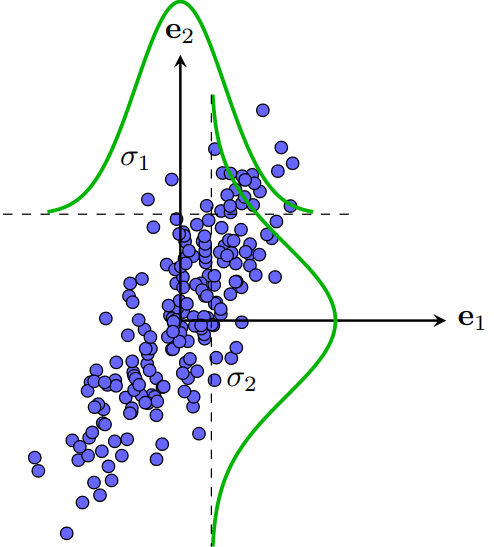
\includegraphics[width=0.8\linewidth]{pca_var.png}
		\caption{}
		\label{fig:27_2c}
	\end{subfigure}
	\caption{
		Ví dụ về kỳ vọng và phương sai. (a) Dữ liệu trong không gian
		một chiều. (b) Dữ liệu trong không gian hai chiều mà hai chiều
		không tương quan. Trong trường hợp này, ma trận hiệp phương sai là ma trận
		đường chéo với hai phần tử trên đường chéo  là $\sigma_1, \sigma_2$, đây
		cũng chính là hai trị riêng của ma trận hiệp phương sai và là phương sai
		của mỗi chiều dữ liệu. (c) Dữ liệu trong không gian hai chiều có tương
		quan. Theo mỗi chiều, ta có thể tính được kỳ vọng và phương sai. Phương sai
		càng lớn thì dữ liệu trong chiều đó càng phân tán. Trong ví dụ này, dữ liệu
		theo chiều thứ hai phân tán nhiều hơn so với chiều thứ nhất. }
	\label{fig:27_2}
\end{figure}

\subsection{Ma trận hiêp phương sai}

Cho $N$ điểm dữ liệu được biểu diễn bởi các vector cột $\mathbf{x}_1, \dots, \mathbf{x}_N$, khi đó, {vector kỳ vọng} và {ma trận hiệp phương sai} của toàn bộ dữ liệu được định nghĩa là
\begin{eqnarray} 
	\bar{\mathbf{x}} &=& \frac{1}{N} \sum_{n=1}^N \mathbf{x}_n, \\\ 
	\mathbf{S} &=&  \frac{1}{N}\sum_{n=1}^N (\mathbf{x}_n - \bar{\mathbf{x}})(\mathbf{x}_n - \bar{\mathbf{x}})^T = \frac{1}{N}\hat{\mathbf{X}}\hat{\mathbf{X}}^T.
\end{eqnarray} 
Trong đó $\hat{\mathbf{X}}$ được tạo bằng cách trừ mỗi cột của $\mathbf{X}$ đi $\bar{\mathbf{x}}$: 
\begin{equation} 
	\hat{\mathbf{x}}_n = \mathbf{x}_n - \bar{\mathbf{x}}.
\end{equation} 
\newpage 
Một vài tính chất của ma trận hiệp phương sai: 
\begin{enumerate}
	
	\item Ma trận hiệp phương sai là một ma trận đối xứng, hơn nữa, nó là một ma trận.
	
	\item Mọi phần tử trên đường chéo của ma trận hiệp phương sai là các số không âm. Chúng chính là phương sai của từng chiều dữ liệu. 
	
	\item Các phần tử ngoài đường chéo $s_{ij}, i \neq j$ thể hiện sự tương quan
	giữa thành phần thứ $i$ và thứ $j$ của dữ liệu, còn được gọi là hiệp phương
	sai. Giá trị này có thể dương, âm hoặc bằng không. Khi nó bằng không, ta nói
	rằng hai thành phần $i, j$ trong dữ liệu là \textit{không tương quan}.
	
	\item Nếu ma trận hiệp phương sai là ma trận đường chéo, ta có dữ liệu hoàn toàn không tương quan giữa các chiều. 
\end{enumerate}

Ví dụ về sự tương quan của dữ liệu được cho trong Hình~\ref{fig:27_2b} và
\ref{fig:27_2c}.% <hr> 
\chapter{ PHÂN TÍCH GIÁ TRỊ KÌ DỊ }

Trong chương này, chúng tôi trình bày cơ sở của phân tích giá trị kì dị của ma trận, thuật toán phân tích giá trị kì dị, và trình bày một số tính chất của ma trận liên quan đến phân tích giá trị kì dị của nó. 
\section{Giới thiệu}
Phân tích giá trị kì dị (SVD) là một trong những phân tích rất quan trọng của ma trận, có nhiều ứng dụng trong khoa học và kĩ thuật. Dạng cổ điển nhất của phân tích giá trị kì dị được phát hiện trong lĩnh vực Hình học vi phân. Vào năm 1873 và 1874 , hai nhà toán học Eugenio Beltrami và Camille Jordan đã độc lập đưa ra giá trị kì dị của dạng song tuyến tính. Năm 1889, James Joshept Sylvester đã đưa ra phân tích giá trị kì dị của ma trận vuông. Đến năm 1915, nhà toán học Autonne phát hiện ra phân tích giá trị kì dị dưới dạng phân tích cực. Năm 1936, hai nhà toán học Carl Eckart và Gale Young đã lần đầu tiên chứng minh phân tích giá trị kì dị đối với ma trận hình chữ nhật thực [] và ma trận vuông phức []. Trong chương này, chúng tôi sẽ tìm hiểu về phân tích giá trị kì dị cho một ma trận hình chữ nhật thực $\mathbf{A}$ cỡ $m \times n$.
\section{Phân tích giá trị kì dị}
Để phát biểu và chứng minh định lý phân tích giá trị kì dị, chúng ta sẽ cần định lí sau đây.

\begin{dl} \label{dl_1} Cho A là một ma trận có cấp $m \times n$. Khi đó, mọi giá trị riêng của ma trận $\mathbf{A}^{T} \mathbf{A}$ đều không âm.
\end{dl}
\begin{proof}
Dễ thấy $\mathbf{A}^{T} \mathbf{A}$ là một ma trận đối xứng. Theo định lí \ref{dlpho}, mọi giá trị riêng của $\mathbf{A}^{T} \mathbf{A}$ đều là số thực. Với mỗi giá trị riêng $\lambda$ của $\mathbf{A}^{T} \mathbf{A}$, giả sử $\mathbf{v}$ là véc tơ riêng tương ứng. Khi đó
\begin{equation} \label{eq1}
\mathbf{A}^{T} \mathbf{A} \mathbf{v}=\lambda \mathbf{v}
\end{equation}
Để ý rằng ta có thể chọn $\mathbf{v}$ là véc tơ đơn vị, i.e. $\|\mathbf{v}\|=1$. Với cách chọn như vậy, ta nhận được

\begin{equation} \label{eq2}
\|\mathbf{A} \mathbf{v}\|^{2}=\langle\mathbf{A} \mathbf{v}, \mathbf{A v}\rangle=(\mathbf{A v})^{T}(\mathbf{A v})=\mathbf{v}^{T} \mathbf{A}^{T} \mathbf{A} \mathbf{v}=\lambda \mathbf{v}^{T} \mathbf{v}=\lambda\|\mathbf{v}\|^{2}=\lambda
\end{equation}

Do vậy, $\lambda \geqslant 0$.
\end{proof}
Ta có định nghĩa và cách xác định các giá trị kì dị của một ma trận như sau


\begin{dn}\rm Cho ma trận $\mathbf{A}$ cỡ $m \times n$ bất kì $(m \leqslant n)$ và $\lambda_{1}, \lambda_{2} \ldots, \lambda_{r}$, $1 \leqslant r \leqslant \min (m, n)$, lần lượt là các giá trị riêng của ma trận $\mathbf{A}^{T} \mathbf{A}$. Các giá trị $\sigma_{i}=\sqrt{\lambda_{i}}, 1 \leqslant i \leqslant r$, được gọi là các giá trị kì dị của ma trận $\mathbf{A}$.

Định lí sau cho ta sự tồn tại của SVD của một ma trận bất kỳ
\end{dn}

\begin{dl}Mọi ma trận $\mathrm{A}$ cỡ $m \times n$ bất kì đều có phân tích SVD có dạng

\begin{equation} \label{eq3}
\mathbf{A}=\mathbf{U D V}^{T}
\end{equation}
trong đó $\mathbf{U}$ và $\mathbf{V}$ lần lượt là các ma trận trực giao cấp $m$ và $n$,\\
$\mathbf{D}$ là ma trận đường chéo cỡ $m \times n$ có dạng

$$
\mathbf{D}=\left[\begin{array}{ccccccc}
	\sigma_{1} & 0 & 0 & \ldots & 0 & \ldots & 0 \\
	0 & \sigma_{2} & 0 & \ldots & 0 & \ldots & 0 \\
	\vdots & \vdots & \ddots & \ldots & \vdots & \ldots & \vdots \\
	0 & 0 & \ldots & \sigma_{r} & 0 & \ldots & 0 \\
	0 & \ldots & \ldots & 0 & 0 & \ldots & 0
\end{array}\right]=\left[\begin{array}{cccc}
	\mathbf{D}_{r \times r} & 0 & \ldots & 0 \\
	0 & \ldots & \ldots & 0 \\
	\vdots & \ddots & & \vdots \\
	0 & \ldots & \ldots & 0
\end{array}\right]
$$
\end{dl}
\begin{proof}
Vì $\mathbf{A}^{T} \mathbf{A}$ là ma trận đối xứng nên theo Định lí \ref{dl_1} $n$ giá trị riêng $\lambda_{1}, \ldots, \lambda_{n}$ của nó đều không âm. Do đó tồn tại $r \leqslant n$ sao cho $\lambda_{1} \geqslant \lambda_{2} \geqslant \lambda_{r}>0$ và $\lambda_{j}=0$ với $j>r$. Khi đó ma trận $\mathbf{A}$ có các giá trị kì dị là $\sigma_{1} \geqslant \sigma_{2} \geqslant \cdots \geqslant \sigma_{r} \geqslant 0$, và $\sigma_{j}=0$ với $j>r$.

Chọn $\mathbf{v}_{i} \in \mathbb{R}^{n}, i=1,2, \ldots, n$, là các vetor riêng tương ứng với $\lambda_{i}$ sao cho $\mathbf{v}_{i}$ là các vetor đơn vị. Đặt $\mathbf{V}=\left(\mathbf{v}_{1}, \mathbf{v}_{2}, \ldots, \mathbf{v}_{n}\right)$, với $\mathbf{v}_{i}$ là các vector cột. Khi đó $\mathbf{V}$ là ma trận trực giao.

Với $\sigma_{i}, 1 \leqslant i \leqslant r$, là các giá trị kì dị dương của $\mathbf{A}$, đặt $\mathbf{u}_{i}=\frac{\mathbf{A v}_{i}}{\sigma_{i}}, i=1,2, \ldots, r$. Khi đó $\mathbf{u}_{i}$ là vector đơn vị trong $\mathbb{R}^{m}$.

Xây dựng ma trận $\mathbf{U}=\left(\mathbf{u}_{1}, \mathbf{u}_{2}, \ldots, \mathbf{u}_{m}\right)$, với $\mathbf{u}_{j}=0, r<j \leqslant m$. Ta có $\mathbf{U}$ là ma trận trực giao.

Ta chứng minh $\mathbf{A}=\mathbf{U D V}^{T}$, hay $\mathbf{A V}=\mathbf{U D}$.

Ta có

$$
\begin{aligned}
	\mathbf{A} \mathbf{V} & =\mathbf{A}\left[\mathbf{v}_{1}, \mathbf{v}_{2}, \ldots, \mathbf{v}_{n}\right]=\left[\mathbf{A v}_{1}, \mathbf{A v}_{2}, \ldots, \mathbf{A} \mathbf{v}_{n}\right]\\
	&=\left[\mathbf{A v}_{1}, \mathbf{A v}_{2}, \ldots, \mathbf{A v}_{r}, 0, \ldots, 0\right] \\
	& =\left[\sigma_{1} \mathbf{u}_{1}, \sigma_{2} \mathbf{u}_{2}, \ldots, \sigma_{r} \mathbf{u}_{r}, 0, \ldots, 0\right]=\left[\mathbf{u}_{1}, \mathbf{u}_{2}, \ldots, \mathbf{u}_{m}\right] \cdot \operatorname{diag}\left(\sigma_{1}, \sigma_{2}, \ldots, \sigma_{r}\right) \\
	& =\mathbf{U D}
\end{aligned}
$$

Vậy $\mathbf{A}=\mathbf{U D V}^{T}$\\%Các vector cột $\mathbf{u}_{i}$ trong ma trận $\mathbf{U}$ được gọi là các vector kì dị trái của $\mathbf{A}$. Các vetor cột $\mathbf{v}_{i}$ trong ma trận $\mathbf{V}$ được gọi là các vector kì dị phải của $\mathbf{A}$.
Trong trường hợp $\operatorname{rank}(\mathbf{A})=r<n$, thì SVD của $\mathbf{A}$ có dạng "chặt cụt" như sau:
$$
\mathbf{A}=\mathbf{U}_r \mathbf{D}_r \mathbf{V}_r^T
$$
trong đó $\mathbf{U}_r, \mathbf{V}_r$ lần lượt là ma trận được tạo bởi $r$ cột đầu tiên của $\mathbf{U}, \mathbf{V}$, và $\mathbf{D}_r$ là ma trận con cấp $r \times r$ được tạo bởi $r$ hàng đầu tiên và $r$ cột đầu tiên của $\mathbf{D}$. Khai triển
như trên được gọi là phân tích SVD "chặt cụt" của $\mathbf{A}$.
\end{proof}
\begin{dl}[\textbf{Về dạng khai triển của phân tích giá trị kì dị}] Cho $\mathbf{A}$ là ma trận cỡ $m \times n$ bất kì. Khi đó
\begin{equation} \label{eq_4}
\mathbf{A}=\mathbf{U D V}^{T}=\sigma_{1} \mathbf{u}_{1} \mathbf{v}_{1}^{T}+\sigma_{2} \mathbf{u}_{2} \mathbf{v}_{2}^{T}+\cdots+\sigma_{r} \mathbf{u}_{r} \mathbf{v}_{r}^{T}
\end{equation}
trong đó $\sigma_{i}$ là các giá trị kì dị dương của ma trận $\mathbf{A}, \mathbf{u}_{i}$ là các vector kì dị trái và $\mathbf{v}_{i}$ là các vector kì dị phải của ma trận $\mathbf{A}$.
\end{dl}
\begin{proof}
Ta có

$$
\begin{aligned}
	& \mathbf{U D V}^{T}=\left[\mathbf{u}_{1}, \mathbf{u}_{2}, \ldots, \mathbf{u}_{m}\right]\left[\begin{array}{ccc}
		\mathbf{D}_{r \times r} & \ldots & 0 \\
		\vdots & \ldots & \vdots \\
		0 & \ldots & 0
	\end{array}\right]\left[\begin{array}{c}
		\mathbf{v}_{1}^{T} \\
		\mathbf{v}_{2}^{T} \\
		\vdots \\
		\mathbf{v}_{n}^{T}
	\end{array}\right] \\
	& =\left[\mathbf{u}_{1}, \mathbf{u}_{2}, \ldots, \mathbf{u}_{r}, \mathbf{u}_{r+1}, \ldots, \mathbf{u}_{m}\right]\left[\begin{array}{ccc}
		\mathbf{D}_{r \times r} & \ldots & 0 \\
		\vdots & \ddots & \vdots \\
		0 & \ldots & 0
	\end{array}\right]\left[\begin{array}{c}
		\mathbf{v}_{1}^{T} \\
		\mathbf{v}_{2}^{T} \\
		\vdots \\
		\mathbf{v}_{r}^{T} \\
		\mathbf{v}_{r+1}^{T} \\
		\vdots \\
		\mathbf{v}_{n}^{T}
	\end{array}\right] \\
	& \left.=\left[\mathbf{u}_{1}, \mathbf{u}_{2}, \ldots, \mathbf{u}_{r}\right]\left[\begin{array}{ccc}
		\sigma_{1} & \ldots & 0 \\
		\vdots & \ddots & \vdots \\
		0 & \ldots & \sigma_{r}
	\end{array}\right]\left[\begin{array}{c}
		\mathbf{v}_{1}^{T} \\
		\mathbf{v}_{2}^{T} \\
		\vdots \\
		\mathbf{v}_{r}^{T}
	\end{array}\right]+\left[\begin{array}{llll}
		\mathbf{u}_{r+1} & \mathbf{u}_{r+2} & \ldots & \mathbf{u}_{m}
	\end{array}\right]\right][0]\left[\begin{array}{c}
		\mathbf{v}_{1}^{T} \\
		\mathbf{v}_{2}^{T} \\
		\vdots \\
		\mathbf{v}_{n}^{T}
	\end{array}\right] \\
	& =\left[\mathbf{u}_{1}, \mathbf{u}_{2}, \ldots, \mathbf{u}_{r}\right]\left[\begin{array}{ccc}
		\sigma_{1} & \ldots & 0 \\
		\vdots & \ddots & \vdots \\
		0 & \ldots & \sigma_{r}
	\end{array}\right]\left[\begin{array}{c}
		\mathbf{v}_{1}^{T} \\
		\mathbf{v}_{2}^{T} \\
		\vdots \\
		\mathbf{v}_{r}^{T}
	\end{array}\right] \\
	& =\left[\sigma_{1} \mathbf{u}_{1}, \ldots, \sigma_{r} \mathbf{u}_{r}\right]\left[\begin{array}{c}
		\mathbf{v}_{1}^{T} \\
		\mathbf{v}_{2}^{T} \\
		\vdots \\
		\mathbf{v}_{r}^{T}
	\end{array}\right]=\sigma_{1} \mathbf{u}_{1} \mathbf{v}_{1}^{T}+\sigma_{2} \mathbf{u}_{2} \mathbf{v}_{2}^{T}+\cdots+\sigma_{r} \mathbf{u}_{r} \mathbf{v}_{r}^{T} .
\end{aligned}
$$
\end{proof}

\section{Thuật toán tìm SVD của một ma trận}
Cho $\mathbf{A}$ là ma trận cỡ $m \times n$, với $m \geq n$. Để tìm $\mathrm{SVD}$ của ma trận $\mathbf{A}$, chúng ta thực hiện các bước sau:
\begin{itemize}

 \item Bước 1. Tính ma trận $\mathbf{A}^{T} \mathbf{A}$ và giải phương trình $\operatorname{det}\left(\mathbf{A}^{T} \mathbf{A}-\lambda \mathbf{I}\right)=0$ để tìm các giá trị riêng $\lambda_{1} \geq \lambda_{2} \geq \ldots \geq \lambda_{n} \geq 0$ của ma trận $\mathbf{A}^{T} \mathbf{A}$. Từ đó suy ra các giá trị kì dị của $\mathbf{A}$ là $\sigma_{i}=\sqrt{\lambda_{i}}, i=\overline{1, n}$ và $\mathbf{D}=\operatorname{diag}\left(\sigma_{1}, \sigma_{2}, \ldots, \sigma_{n}\right)$

\item Bước 2. Tương ứng với mỗi giá trị riêng $\lambda_{i}$, tìm véctơ riêng $\mathbf{v}_{i} \in \mathbb{R}^{n}$ sao cho $\left(\mathbf{A}^{T} \mathbf{A}-\lambda \mathbf{I}\right) v_{i}=0$. Từ đó tìm được ma trận trực giao $\mathbf{V}$ cấp $n$ chứa các véctơ kì dị phải của $\mathbf{A}$.

\item Bước 3. Xác định các véctơ kì dị trái của $\mathbf{A}$ theo công thức

$$
\mathbf{u}_{i}=\frac{1}{\sigma_{i}} \mathbf{A} \mathbf{v}_{i}
$$

Bổ sung $n-r$ vector $\mathbf{u}_{r+1}, \ldots, \mathbf{u}_{n}$ vào hệ $\left\{\mathbf{u}_{1}, \mathbf{u}_{2}, \ldots, \mathbf{u}_{r}\right\}$ sao cho $\left\{\mathbf{u}_{1},\mathbf{u}_{2}, \ldots, \mathbf{u}_{n}\right\}$ lập thành một cơ sở trực chuẩn của $\mathbb{R}^{n}$. Từ đó nhận được ma trận trực giao $\mathbf{U}$ chứa các véctơ kì dị trái của $\mathbf{A}$, và

$$
\mathbf{A}=\mathbf{U D V}^{T}
$$
là phân tích SVD của ma trận $\mathbf{A}$.
\end{itemize}
\subsubsection{Ví dụ}

Tìm SVD của ma trận $\mathbf{A}=\left[\begin{array}{ll}1 & 0 \\ 1 & 0 \\ 0 & 1\end{array}\right]$.

Lời giải:

Bước 1: Tìm các giá trị kì dị củ ma trận $\mathbf{A}$

Ta có

$$
\mathbf{A}^{T} \mathbf{A}=\left[\begin{array}{lll}
	1 & 1 & 0 \\
	0 & 0 & 1
\end{array}\right]\left[\begin{array}{ll}
	1 & 0 \\
	1 & 0 \\
	0 & 1
\end{array}\right]=\left[\begin{array}{ll}
	2 & 0 \\
	0 & 1
\end{array}\right]
$$

Giải phương trình $\operatorname{det}\left(\mathbf{A}^{T} \mathbf{A}-\lambda \mathbf{I}\right)=0$, ta tìm đượccác giá trị riêng $\lambda$ của $\mathbf{A}^{T} \mathbf{A}$ là $\lambda_{1}=2, \lambda_{2}=1$. Do đó các giá trị kì dị của $\mathbf{A}$ là $\sigma_{1}=\sqrt{2}, \sigma_{2}=1$. Suy ra

$$
\mathbf{D}=\left[\begin{array}{cc}
	\sqrt{2} & 0 \\
	0 & 1
\end{array}\right]
$$

Bước 2: Tìm ma trận $\mathbf{V}$

Giải phương trình $\left(\mathbf{A}^{T} \mathbf{A}-\lambda \mathbf{I}\right) \mathbf{v}=0$ ta tìm được các véctơ riêng tương ứng là \\
$\mathbf{v}_{1}=\left[\begin{array}{l}1 \\ 0\end{array}\right]$ và $\mathbf{v}_{2}=\left[\begin{array}{l}0 \\ 1\end{array}\right]$.

Từ đó suy ra

$$
\mathbf{V}^{T}=\left[\begin{array}{ll}
	1 & 0 \\
	0 & 1
\end{array}\right]
$$

Bước 3: Tìm ma trận $\mathbf{U}$

Ta có

$$
\mathbf{u}_{1}=\frac{1}{\sigma_{1}} \mathbf{A} \mathbf{v}_{1}=\frac{1}{\sqrt{2}}\left[\begin{array}{ll}
	1 & 0 \\
	1 & 0 \\
	0 & 1
\end{array}\right]\left[\begin{array}{l}
	1 \\
	0
\end{array}\right]=\left[\begin{array}{c}
	\frac{1}{\sqrt{2}} \\
	\frac{1}{\sqrt{2}} \\
	0
\end{array}\right]
$$

và

$$
\mathbf{u}_{2}=\frac{1}{\sigma_{2}} \mathbf{A} \mathbf{v}_{1}=\left[\begin{array}{ll}
	1 & 0 \\
	1 & 0 \\
	0 & 1
\end{array}\right]\left[\begin{array}{l}
	0 \\
	1
\end{array}\right]=\left[\begin{array}{l}
	0 \\
	0 \\
	1
\end{array}\right]
$$

Do đó

$$
\mathbf{U}=\left[\begin{array}{cc}
	\frac{1}{\sqrt{2}} & 0 \\
	\frac{1}{\sqrt{2}} & 0 \\
	0 & 1
\end{array}\right]
$$

Vậy phân tích SVD của ma trận $\mathbf{A}$ là

$$
\mathbf{A}=\left[\begin{array}{ll}
	1 & 0 \\
	1 & 0 \\
	0 & 1
\end{array}\right]=\left[\begin{array}{cc}
	\frac{1}{\sqrt{2}} & 0 \\
	\frac{1}{\sqrt{2}} & 0 \\
	0 & 1
\end{array}\right]\left[\begin{array}{cc}
	\sqrt{2} & 0 \\
	0 & 1
\end{array}\right]\left[\begin{array}{ll}
	1 & 0 \\
	0 & 1
\end{array}\right]
$$
Bên dưới là ví dụ về SVD trên PYTHON3.
\begin{figure}[htp]
	\centering
	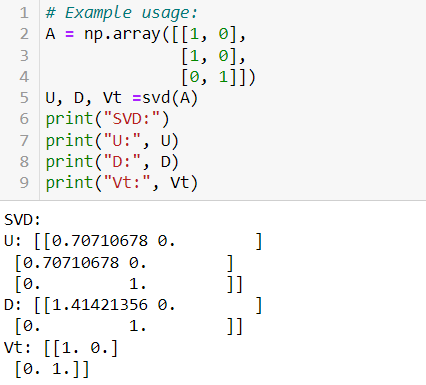
\includegraphics[scale=0.9]{example_svd.png}
	\caption{Ví dụ SVD trên PYTHON3}
	\label{fig:galaxy}
\end{figure}

\section{Một số tính chất của ma trận liên quan đến SVD của nó}
\begin{dl}
Cho ma trận $\mathbf{A}$ cỡ $m \times n$ bất kì, có phân tích SVD là

$$
\mathbf{A}=\mathbf{U D V}^{T}
$$
Khi đó, hạng của $\mathbf{A}$ đúng bằng số các giá trị kì dị dương của $\mathbf{A}$.
\end{dl}
\begin{proof} 
Giả sử $r$ là số các giá trị kì dị dương của $\mathbf{A}$. Đặt $\mathbf{U}_{r}=\left[\mathbf{u}_{1}, \mathbf{u}_{2}, \ldots, \mathbf{u}_{r}\right]$, $\mathbf{V}_{r}=\left[\mathbf{v}_{1}, \mathbf{v}_{2}, \ldots, \mathbf{v}_{r}\right]$. Do tính chất của hạng của ma trận và tính trực giao của $\mathbf{U}, \mathbf{V}$ ta suy ra
$$
\begin{aligned}
	& \operatorname{rank}\left(\mathbf{U}_{r}\right)=\operatorname{rank}\left(\mathbf{U}_{r} \mathbf{U}_{r}^{T}\right)=\operatorname{rank}\left(\mathbf{I}_{r}\right)=r, \\
	& \operatorname{rank}\left(\mathbf{V}_{r}^{T}\right)=\operatorname{rank}\left(\mathbf{V}_{r}^{T} \mathbf{V}_{r}\right)=\operatorname{rank}\left(\mathbf{I}_{r}\right)=r .
\end{aligned}
$$
Do đó
$$
\operatorname{rank}(\mathbf{A})=\operatorname{rank}\left(\mathbf{U D V}^{T}\right)=\operatorname{rank}\left(\mathbf{U}_{r} \mathbf{D} \mathbf{V}_{r}^{T}\right)=\operatorname{rank}\left(\mathbf{D V}_{r}^{T}\right)=\operatorname{rank}(\mathbf{D})=r$$
\end{proof}
\begin{dl} 
Cho $\mathbf{A}$ là một ma trận có cỡ $m \times n$. Giả sử $\mathbf{A}$ có phân tích $\mathrm{SVD}$ dưới dạng khai triển là

$$
\mathbf{A}=\sigma_{1} \mathbf{u}_{1} \mathbf{v}_{1}^{T}+\cdots+\sigma_{r} \mathbf{u}_{r} \mathbf{v}_{r}^{T}
$$
Khi đó, với mỗi số nguyên dương $k<r$, ma trận
$$
\mathbf{A}_{k}=\sigma_{1} \mathbf{u}_{1} \mathbf{v}_{1}^{T}+\cdots+\sigma_{k} \mathbf{u}_{k} \mathbf{v}_{k}^{T}
$$
có hạng $k, \operatorname{rank}\left(\mathbf{A}_{k}\right)=k$.
\end{dl}
\begin{proof}
Dễ thấy rằng ma trận $\mathbf{A}_{k}$ có thể viết ở dạng

$$
\mathbf{A}_{k}=\left(\sigma_{1} \mathbf{v}_{1}^{T}+\cdots+\sigma_{k} \mathbf{v}_{k}^{T}\right)\left[\begin{array}{c}
	\mathbf{u}_{1} \\
	\mathbf{u}_{2} \\
	\vdots \\
	\mathbf{u}_{k}
\end{array}\right]
$$

Ta có

$$
\left[\begin{array}{c}
	\mathbf{u}_{1} \\
	\mathbf{u}_{2} \\
	\vdots \\
	\mathbf{u}_{k}
\end{array}\right]\left[\begin{array}{c}
	\mathbf{u}_{1} \\
	\mathbf{u}_{2} \\
	\vdots \\
	\mathbf{u}_{k}
\end{array}\right]^{T}=\mathbf{I}_{k} \text { và rank }\left[\begin{array}{c}
	\mathbf{u}_{1} \\
	\mathbf{u}_{2} \\
	\vdots \\
	\mathbf{u}_{k}
\end{array}\right]=\operatorname{rank}\left[\begin{array}{c}
	\mathbf{u}_{1} \\
	\mathbf{u}_{2} \\
	\vdots \\
	\mathbf{u}_{k}
\end{array}\right]\left[\begin{array}{c}
	\mathbf{u}_{1} \\
	\mathbf{u}_{2} \\
	\vdots \\
	\mathbf{u}_{k}
\end{array}\right]^{T}=k .
$$

Xét $\operatorname{rank}\left(\sigma_{1} \mathbf{v}_{1}^{T}, \sigma_{2} \mathbf{v}_{2}^{T}, \ldots, \sigma_{k} \mathbf{v}_{k}^{T}\right)$. Ta có

$$
\left(\mathbf{v}_{1}^{T}, \mathbf{v}_{2}^{T}, \ldots, \mathbf{v}_{k}^{T}\right)\left(\mathbf{v}_{1}, \mathbf{v}_{2}, \ldots, \mathbf{v}_{k}\right)=\mathbf{I}_{k}
$$

Do đó

$$
\left(\sigma_{1} \mathbf{v}_{1}^{T}, \ldots, \sigma_{k} \mathbf{v}_{k}^{T}\right)\left(\mathbf{v}_{1}, \mathbf{v}_{2}, \ldots, \mathbf{v}_{k}\right)=\left[\begin{array}{c}
	\sigma_{1} \\
	\sigma_{2} \\
	\vdots \\
	\sigma_{k}
\end{array}\right] \mathbf{I}_{k}=\left[\begin{array}{cccc}
	\sigma_{1} & 0 & \ldots & 0 \\
	0 & \sigma_{2} & \ldots & 0 \\
	\vdots & \vdots & \ddots & \vdots \\
	0 & 0 & \ldots & \sigma_{k}
\end{array}\right]=\mathbf{B}
$$

Vì  $\operatorname{rank}(\mathbf{B})=k=\operatorname{rank}\left(\mathbf{v}_{1}, \mathbf{v}_{2}, \ldots, \mathbf{v}_{k}\right)$ nên

$$
\operatorname{rank}\left(\sigma_{1} \mathbf{v}_{1}^{T}, \sigma_{2} \mathbf{v}_{2}^{T}, \ldots, \sigma_{k} \mathbf{v}_{k}^{T}\right)=k
$$

Từ đó, ta suy $\operatorname{ra~} \operatorname{rank}\left(\mathbf{A}_{k}\right)=k$.
\end{proof}
\begin{dl} 
 Cho $\mathbf{A}$ là ma trận cỡ $m \times n$ bất kì và $\sigma_{1}, \sigma_{2}, \ldots, \sigma_{r}$ là các giá trị kì dị dương của $\mathbf{A}$. Khi đó $\|\mathbf{A}\|_{F}=\sqrt{\sigma_{1}^{2}+\sigma_{2}^{2}+\cdots+\sigma_{r}^{2}}$.
\end{dl} 
\begin{proof}
Giả sử $\mathbf{Q}$ là ma trận trực giao cấp $m$. Khi đó
\begin{align*}
\|\mathbf{Q} \mathbf{A}\|_{F}^{2}&=\left\|\left[\mathbf{Q} \mathbf{a}_{1}, \ldots, \mathbf{Q} \mathbf{a}_{n}\right]\right\|_{F}^{2}\\
&=\left\|\mathbf{Q}_{\mathbf{1}}\right\|_{F}^{2}+\cdots+\left\|\mathbf{Q} \mathbf{a}_{n}\right\|_{F}^{2}\\
&=\left\|\mathbf{a}_{1}\right\|_{F}^{2}+\cdots+\left\|\mathbf{a}_{n}\right\|_{F}^{2}=\|\mathbf{A}\|_{F}^{2}.
\end{align*}
Giả sử $\mathbf{A}$ có phân tích $\mathrm{SVD}$ là $\mathbf{A}=\mathbf{U D V}^{T}$. Vì $\mathbf{U}$ và $\mathbf{V}$ là các ma trận trực giao nên
$$
\left.\|\mathbf{A}\right\|_{F}^{2}=\left\|\mathbf{U D V}^{T}\right\|_{F}^{2}=\left\| \mathbf{D V}^{T}\right\|_{F}^{2}=\left\|\left(\mathbf{D V}^{T}\right)^{T}\right\|_{F}^{2}=\left\| \mathbf{V D}^{T}\right\|_{F}^{2}=\left\| \mathbf{D}^{T}\right \|_{F}^{2}=\sigma_{1}^{2}+\sigma_{2}^{2}+\cdots+\sigma_{r}^{2}
$$

Vậy

$$
\|\mathbf{A}\|_{F}^{2}=\sqrt{\sigma_{1}^{2}+\cdots+\sigma_{r}^{2}}
$$

với $\sigma_{i}, i=1,2, \ldots, r$ là các giá trị kì dị của ma trận $\mathbf{A}$.
\end{proof} 
%\section{Phân tích thành phần chính (PCA)}
\chapter{ Phân tích thành phần chính }
\section{Giới thiệu}
%%Phép phân tích thành phần chính (Principal Components Analysis - PCA) là một thuật toán thống kê sử dụng phép biến đổi trực giao để biến đổi một tập hợp dữ liệu từ một không gian nhiều chiều sang một không gian mới ít chiều hơn (2 hoặc 3 chiều) nhằm tối ưu hóa việc thể hiện sự biến thiên của dữ liệu.
%%Trong công tác nghiên cứu thực nghiệm, ta thu thập được những bộ dữ liệu thường được thể hiện dưới dạng bảng các giá trị số của nhiều cá thể. Chúng tạo thành “đám mây số liệu” khá phức tạp và việc tìm hiểu thông tin từ đó gặp khó khăn. Một trong những phương pháp hiệu quả trong xử lý số liệu nhiều chiều là phương pháp phân tích thành phần chính – Principal component analysis (PCA). Đây là một thuật toán thống kê sử dụng phép biến đổi trực giao để biến đổi một tập hợp dữ liệu từ một không gian nhiều chiều sang một không gian mới ít chiều hơn (2 hoặc 3 chiều) nhằm tối ưu hóa việc thể hiện sự biến thiên của dữ liệu. PCA được áp dụng để phân tích dữ liệu trong rất nhiều lĩnh vực như nông nghiệp, kinh tế, y tế và các ngành khoa học khác.
Phép phân tích thành phần chính (Principal Components Analysis - PCA) là một phương pháp phân tích ma trận đa biến, giúp giảm số chiều của dữ liệu bằng cách tìm ra các thành phần chính của ma trận đó. Ý tưởng của PCA là chuyển đổi dữ liệu ban đầu từ không gian có số chiều cao sang không gian có số chiều thấp hơn, giúp cho việc xử lý và phân tích dữ liệu dễ dàng hơn.
Phép phân tích thành phần chính được đưa ra vào năm 1901 bởi Karl Pearson và đã được phát triển và ứng dụng rộng rãi trong nhiều lĩnh vực khác nhau như nhận dạng hình ảnh, phân tích tín hiệu, dự báo kinh tế và thị trường tài chính.

Một trong những ứng dụng quan trọng nhất của phép phân tích thành phần chính là giảm số chiều của dữ liệu. Khi dữ liệu có số chiều lớn, việc phân tích và xử lý trở nên phức tạp và tốn nhiều thời gian. Đồng thời cho phép giảm số chiều của dữ liệu bằng cách xác định các thành phần chính của ma trận, giúp cho việc xử lý và phân tích dữ liệu trở nên đơn giản và nhanh chóng hơn.

Ngoài ra, phép phân tích này còn được sử dụng để giảm tác động của nhiễu trong dữ liệu, phát hiện các mối quan hệ giữa các biến đầu vào và giúp tối ưu hóa các thuật toán máy học.

Với những ứng dụng và lợi ích của mình, phép phân tích thành phần chính đã trở thành một công cụ quan trọng trong phân tích dữ liệu và được sử dụng rộng rãi trong nhiều lĩnh vực khác nhau.
\section{Ý tưởng}
Giả sử dữ liệu ban đầu là $\mathbf{x} \in \mathbb{R}^{m}$ và dữ liệu đã được giảm chiều là $\mathbf{z} \in \mathbb{R}^{r}$ với $r<m$. Cách đơn giản nhất để giảm chiều dữ liệu từ $m$ về $r<m$ là chỉ cần giữ lại $r$ phần tử quan trọng nhất. Có hai câu hỏi được đặt ra ở đây:
\begin{itemize}

\item[(i)] Làm thế nào để xác định tầm quan trọng của mỗi chiều dữ liệu?
\item[(ii)] Nếu tầm quan trọng của các chiều dữ liệu là như nhau, ta cần bỏ đi chiều nào?
	
\end{itemize}
 \begin{figure}[t]
	\begin{subfigure}{0.59\textwidth}
		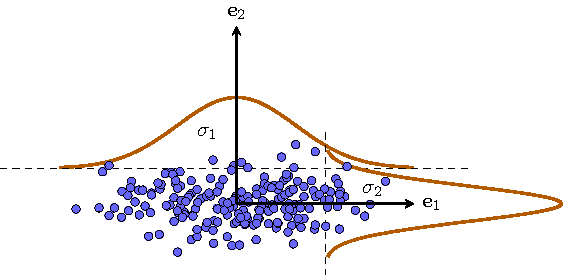
\includegraphics[width=0.99\linewidth]{pca_diagvar.pdf}
		\caption{}
		\label{fig:pca_2a}
	\end{subfigure}
	\begin{subfigure}{0.33\textwidth}
		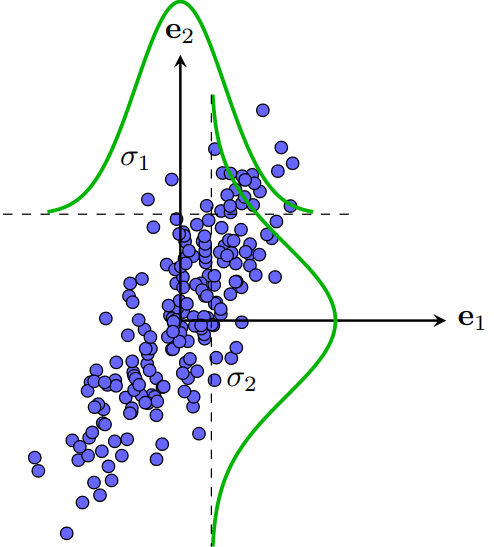
\includegraphics[width=0.99\linewidth]{pca_var.png}
		\caption{}
		\label{fig:pca_2b}
	\end{subfigure}
	\caption{Ví dụ về phương sai của dữ liệu trong không gian hai chiều. (a)
		Phương sai của chiều thử hai (tỉ lệ với độ rộng của đường hình chuông) nhỏ
		hơn phương sai của chiều thứ nhất. (b) Cả hai chiều có phương sai đáng kể. Phương sai của
		mỗi chiều là phương sai của thành phần tương ứng được lấy trên toàn bộ dữ
		liệu. Phương sai tỉ lệ thuận với độ phân tán của dữ liệu.}
	\label{fig:pca_2}
\end{figure}
Giả sử vector dữ liệu ban đầu $\mathbf{x} \in \R^{D}$ được giảm chiều trở thành $\mathbf{z}
\in \R^K$ với $K < D$. Một cách đơn giản để giảm chiều dữ liệu từ $D$ về $K < D$ là chỉ giữ lại $K$ phần tử {quan trọng nhất}. Có hai câu hỏi lập tức
được đặt ra. Thứ nhất, làm thế nào để xác định {tầm quan trọng} của
mỗi phần tử? Thứ hai, nếu tầm quan trọng của các phần tử là như
nhau, ta cần bỏ đi những phần tử nào?

Để trả lời câu hỏi thứ nhất, hãy quan sát Hình \ref{fig:pca_2a}. Giả sử các
điểm dữ liệu có thành phần thứ hai (phương đứng) giống hệt nhau hoặc sai khác
nhau không đáng kể (phương sai nhỏ). Khi đó, thành phần này hoàn toàn có thể được lược
bỏ, và ta ngầm hiểu rằng nó sẽ được xấp xỉ bằng kỳ vọng của thành phần đó
trên toàn bộ dữ liệu. Ngược lại, nếu áp dụng phương pháp này lên chiều thứ nhất (phương ngang), {lượng thông tin} bị mất đi đáng kể do sai số xấp xỉ quá lớn. Vì vậy, lượng thông tin theo mỗi thành phần có thể được đo bằng phương sai của dữ liệu trên thành phần đó. Tổng lượng
thông tin là tổng phương sai trên toàn bộ các thành phần. Lấy
một ví dụ về việc có hai camera được đặt dùng để chụp cùng một người, một camera
phía trước và một camera đặt trên đầu. Rõ ràng, hình ảnh thu được từ
camera đặt phía trước mang nhiều thông tin hơn so với hình ảnh nhìn từ
phía trên đầu. Vì vậy, bức ảnh chụp từ phía trên đầu có thể được bỏ qua mà không
làm mất đi quá nhiều thông tin về hình dáng của người đó.

Câu hỏi thứ hai tương ứng với trường hợp Hình~\ref{fig:pca_2b}. Trong cả hai
chiều, phương sai của dữ liệu đều lớn; việc bỏ đi một trong hai chiều đều khiến
một lượng thông tin đáng kể bị mất đi. Tuy nhiên, nếu xoay trục toạ độ đi một
góc phù hợp, một trong hai chiều dữ liệu có thể được lược bở vì dữ liệu có xu
hướng phân bố xung quanh một đường thẳng.

\textit{Phân tích thành phần chính} (principle component analysis, PCA) là
phương pháp đi tìm một phép xoay trục toạ độ để được một hệ trục toạ độ mới sao
cho trong hệ mới này, thông tin của dữ liệu chủ yếu tập trung ở một vài thành
phần. Phần còn lại chứa ít thông tin hơn có thể được lược bỏ.

\section{Phân tích thành phần chính}

Về mặt hình thức, cho ma trận dữ liệu $\mathbf{X} \in \mathbb{R}^{m \times n}$ với mỗi giá trị đã được chuẩn hóa sao cho mỗi cột có giá trị trung bình là 0. PCA của $\mathbf{X}$ với $r$ thành phần là tìm ma trận trực giao $\mathbf{A} \in \mathbb{R}^{m \times r}$ và ma trận $\mathbf{B} \in \mathbb{R}^{n \times r}$ sao cho $\mathbf{X}$ có thể biểu diễn được dưới dạng ma trận

$$
\mathbf{X}=\mathbf{A} \mathbf{B}^{T}+\mathbf{E}
$$
trong đó $\|\mathbf{E}\|^{2}$ đạt giá trị nhỏ nhất. Ma trận $\mathbf{A}$ được gọi là ma trận thành phần, và các cột của nó là các thành phần chính. Ma trận $\mathbf{B}$ được gọi là ma trận tải, các tải trọng là các trọng số cho phép tái cấu trúc các biến ban đầu dưới dạng tổ hợp tuyến tính của các thành phần chính. Cặp $(\mathbf{A}, \mathbf{B})$ được gọi là nghiệm PCA.
Ngoài ra, PCA được trình bày theo một cách khác dưới dạng véctơ như sau:

$$
\mathbf{X}=\sum_{i=1}^{r} \mathbf{a}_{i} \mathbf{b}_{i}^{T}+\mathbf{E}
$$
%m^{\frac{1}{2}}
Điều này cho thấy $\mathrm{PCA}$ là xấp xỉ $\mathbf{X}$ với tổng của $r$ ma trận có hạng 1.
Mục tiêu của PCA là làm giảm tối thiểu $\|\mathbf{E}\|^{2}=\left\|\mathbf{X}-\mathbf{A} \mathbf{B}^{T}\right\|^{2}$. Vì $\operatorname{rank}\left(\mathbf{A} \mathbf{B}^{T}\right) \leq r$ nên $\mathbf{A} \mathbf{B}^{T}$ là SVD "chặt cụt" của $\mathbf{X}$, nghĩa là nếu $\mathbf{U}_{r} \mathbf{D}_{r}\left(\mathbf{V}_{r}\right)^{T}$ là SVD "chặt cụt" của $\mathbf{X}$ thì $\mathbf{A}= \mathbf{U}_{r}$ và $\mathbf{B}^{T}= \mathbf{D}_{r}\left(\mathbf{V}_{r}\right)^{T}$. Số lượng thành phần tối thiểu phù hợp là số giá trị kì dị khác 0 của $\mathbf{X}$, hay là hạng của $\mathbf{X}$. Vì vậy, không cần thiết phải lấy số thành phần $r$ lớn hơn số lượng biến $n$. Trên thực tế, $r$ thường được lấy nhỏ hơn nhiều so với $n$.

Do thứ tự giảm dần của các giá trị kì dị của $\mathbf{X}$ trong SVD, thành phần chính đầu tiên giải thích phương sai nhiều nhất có thể và từng thành phần chính tiếp theo giải thích phương sai với ràng buộc là nó trực giao (không tương quan với các thành phần trước đó). Khi đó tổng phương sai được giải thích là $\operatorname{Tr}\left(\mathbf{B} \mathbf{B}^{T}\right)=\operatorname{Tr}\left(m^{-\frac{1}{2}} \mathbf{D}_{r}^{2}\right)$ với $\operatorname{Tr}\left(\mathbf{D}_{r}^{2}\right)$ là tổng bình phương của $r$ giá trị kì dị lớn nhất của $\mathbf{X}$.

\section{Tìm các thành phần chính của bài toán PCA thông qua SVD}

Xét một vector $\mathbf{x}$ bất kì. Thành phần chính là tổ hợp tuyến tính $\mathbf{s}=\sum_{i=1}^{m} \mathbf{w}_{i} \mathbf{x}_{i}$ có chứa càng nhiều phương sai của dữ liệu đầu vào càng tốt. Như vậy, thành phần chính đầu tiên được định nghĩa bằng trực giác là tổ hợp tuyến tính của các biến quan sát, trong đó có phương sai lớn nhất.

Chúng ta cần đưa ra ràng buộc cho chuẩn của vectơ $\mathbf{w}=\left(\mathbf{w}_{1}, \mathbf{w}_{2}, \ldots, \mathbf{w}_{m}\right)$. Để đơn giản, chúng ta ràng buộc $\mathbf{w}$ có chuẩn bằng 1 , tức là

$$
\|\mathbf{w}\|=\sqrt{\sum_{i=1}^{m} \mathbf{w}_{i}^{2}}=1
$$

Các ràng buộc khác về giá trị chuẩn của $\mathbf{w}$ chúng ta có thể đưa về ràng buộc trên.
Chú ý rằng phương sai của một tổ hợp tuyến tính bất kì đều có thể được tính thông qua ma trận hiệp phương sai của dữ liệu. Xét một tổ hợp tuyến tính $\mathbf{w}^{T} \mathbf{x}=\sum_{i=1}^{m} w_{i} x_{i}$. Giả sử giá trị trung bình bằng 0 , tức là $E\{\mathbf{x}\}=0$. Khi đó

$$
\begin{aligned}
	E\left\{\left(\mathbf{w}^{T} \mathbf{x}\right)^{2}\right\}&=E\left\{\left(\mathbf{w}^{T} \mathbf{x}\right)\left(\mathbf{w}^{T} \mathbf{x}\right)\right\}\\
	 &=E\left\{\mathbf{w}^{T}\left(\mathbf{x} \mathbf{x}^{T}\right) \mathbf{w}\right\}\\
	 & =\mathbf{w}^{T} E\left\{\mathbf{x} \mathbf{x}^{T}\right\} \\
	& =\mathbf{w}^{T} \mathbf{C} \mathbf{w}
\end{aligned}
$$

trong đó $\mathbf{C}=E\left\{\mathbf{x} \mathbf{x}^{T}\right\}$ là ma trận hiệp phương sai. Vì vậy, bài toán cơ bản $\mathrm{PCA}$ được xác định như sau:

$$
\max _{\mathbf{w}:\|\mathbf{w}\|=1} \mathbf{w}^{T}\mathbf{Cw}
$$

Vì $\mathbf{C}$ là ma trận đối xứng nên theo định lí phổ của ma trận đối xứng, tồn tại ma trận trực giao $\mathbf{U} \in \mathbb{R}^{m \times n}$ và ma trận đường chéo $\mathbf{D}=\operatorname{diag}\left(\lambda_{1}, \ldots, \lambda_{n}\right) \in \mathbb{R}^{n \times n}$ sao cho $\mathbf{C} = \mathbf{U} \mathbf{D} \mathbf{ U}^{T}$, trong đó $\lambda_{1}, \ldots, \lambda_{n}$ là các giá trị riêng của $\mathbf{C}$, và các vector cột của $\mathbf{U}$ là các véctơ riêng của $\mathbf{C}$ ứng với giá trị riêng đó. Thực hiện đổi biến $\mathbf{v}=\mathbf{U}^{T} \mathbf{w}$. Khi đó ta nhận được

$$
\mathbf{w}^{T} \mathbf{C} \mathbf{w}=\mathbf{w}^{T} \mathbf{U} \mathbf{D} \mathbf{U}^{T} \mathbf{w}=\mathbf{v}^{T} \mathbf{D} \mathbf{v}=\sum_{i=1}^{n} \mathbf{v}_{i}^{2} \lambda_{i}
$$

Vì $\mathbf{U}$ trực giao nên $\|\mathbf{v}\|=\|\mathbf{w}\|$, do đó, $\mathbf{v}$ có ràng buộc $\|\mathbf{v}\|=1$. Tiếp tục thực hiện phép đổi biến $\mathbf{m}_{i}=\mathbf{v}_{i}^{2}, i=1, \ldots, n$. Khi đó ràng buộc $\|\mathbf{v}\|=1$ tương đương với ràng buộc $\mathbf{m}_{i} \geq 0$ và $\sum_{i=1}^{n} \mathbf{m}_{i}=1$. Bài toán được chuyển sang dạng

$$
\max \sum_{i=1}^{n} \mathbf{m}_{i} \lambda_{i}, \text { với } \mathbf{m}_{i} \geq 0, \sum_{i=1}^{n} m_{i}=1 \text {. }
$$

Rõ ràng, bài toán cho thấy giá trị lớn nhất tìm được khi $\mathbf{m}_{i}$ tương ứng với $\lambda_{i}$ lớn nhất bằng 1 và các $\mathbf{m}_{i}$ còn lại bằng 0. Kí hiệu $i^{*}$ là chỉ số của giá trị riêng lớn nhất. Trở lại biến $\mathbf{w}$, điều này tương đương với $\mathbf{w}$ bắt đầu từ vectơ riêng thứ $i^{*}$, tức là cột thứ $i^{*}$ của $\mathbf{U}$. Như vậy, thành phần chính đầu tiên được tìm một cách dễ dàng thông qua phân tích giá trị riêng.

Do các vectơ riêng của ma trận đối xứng là trực giao nên việc tìm thành phần chính thứ hai đồng nghĩa với việc tối đa hóa phương sai sao cho $\mathbf{v}_{i^{*}}$ vẫn bằng 0. Điều này thực sự tương đương với việc tạo $\mathbf{w}$ trực giao mới cho vectơ riêng đầu tiên. Như vậy, chúng ta có bài toán tối ưu hóa tương tự nhưng với ràng buộc $\mathbf{m}_{i^{*}}=0$. Rõ ràng, nghiệm của bài toán tối ưu đó thu được khi $\mathbf{w}$ bằng với vector riêng tương ứng với giá trị riêng lớn nhất thứ hai. Logic này áp dụng cho thành phần chính thứ $k$.

Do đó, tất cả các thành phần chính có thể được tìm thấy bằng cách đặt các vector riêng $\mathbf{u}_{i}\text { với } i=1, \ldots, n$ trong $\mathbf{U}$ sao cho các giá trị riêng giảm dần. Chúng ta hãy giả sử $\mathbf{U}$ được định nghĩa như vậy. Khi đó thành phần chính thứ $i$ có dạng

$$
\mathbf{s}_{i}=\mathbf{u}_{i}^{T}\mathbf{ x}
$$
Lưu ý rằng tất cả các $\lambda_{i}$ đều không âm đối với ma trận hiệp phương sai.

\section{Tính duy nhất nghiệm của PCA}

\begin{dl} \label{dl351}
Nếu $(\mathbf{A, B})$ là một nghiệm của mô hình PCA thì $(\mathbf{A Q, B Q})$ cũng là một nghiệm của mô hình PCA, với $\mathbf{Q}$ là ma trận trực giao cấp $r$.

Lúc này, $\mathbf{Q}$ được gọi là phép quay trực giao.
\end{dl}
\begin{proof}
Giả sử $(\mathbf{A, B})$ là một nghiệm của mô hình PCA.
Với $\mathbf{Q}$ là một ma trận trực giao cấp $r$, tức là $\mathbf{Q Q}^{T}=\mathbf{Q}^{T} \mathbf{Q}=\mathbf{I}_{r}$, ta có

$$
(\mathbf{A Q})(\mathbf{A Q})^{T}=\mathbf{A Q Q}^{T} \mathbf{A}^{T}=\mathbf{AI}_{r} \mathbf{A}^{T}=\mathbf{A A}^{T}=\mathbf{I}_{m}
$$

và

$$
(\mathbf{A Q})^{T}(\mathbf{A Q})=\mathbf{Q}^{T} \mathbf{A}^{T} \mathbf{A Q}=\mathbf{Q}^{T} I_{r} \mathbf{Q}=\mathbf{Q}^{T} \mathbf{Q}=\mathbf{I}_{r}
$$
Suy ra $(\mathbf{A Q})$ là ma trận trực giao cỡ $m \times r$.
Mặt khác, ta có

$$
(\mathbf{A Q})(\mathbf{B Q})^{T}=\mathbf{A Q Q}^{T} \mathbf{B}^{T}=\mathbf{A I}_{r} \mathbf{B}^{T}=\mathbf{A B}^{T}
$$

và

$$
\left\|\mathbf{X-A Q Q}^{T} \mathbf{B}^{T}\right\|^{2}=\left\|\mathbf{X-A B}^{T}\right\|^{2}
$$

Vậy $(\mathbf{A Q, B Q})$ là một nghiệm của mô hình PCA.
\end{proof}
Từ Định lí \ref{dl351}, ta có nhận xét sau:\\
Nhận xét: 
\begin{itemize}
\item[(i)] Nghiệm $(\mathbf{A, B})$ của PCA không duy nhất.
\item[(ii)] Phép quay trực giao $\mathbf{Q}$ sẽ cho ta ma trận tải có cấu trúc đơn giản hơn, do đó các nhân tố sẽ được diễn giải dễ dàng hơn.
\end{itemize}
\section{Thuật toán tìm PCA của một ma trận}

Giả sử $\mathbf{X}$ là ma trận cỡ $m \times n$, với $m \geq n$. Để tìm $\mathrm{PCA}$ của ma trận $\mathbf{X}$, chúng ta thực hiện các bước sau:

- Bước 1: Chuẩn hóa dữ liệu sao cho $E\{\mathbf{x_i}\}=0$ với $\mathbf{x_i}$ là vector hàng của của ma trận $\mathbf{X}$

- Bước 2: Tìm SVD "chặt cụt" của ma trận $\mathbf{X}$, ta được $\mathbf{X}=\mathbf{U}_{r} \mathbf{D}_{r}\left(\mathbf{V}_{r}\right)^{T}$ với $r \leq n$.

- Bước 3: Tính ma trận $\mathbf{A}$ và $\mathbf{B}$ theo công thức sau:

$$
\mathbf{A} =  \mathbf{U}_{r}, \quad \mathbf{B}^{T}= \mathbf{D}_{r}\left(\mathbf{V}_{r}\right)^{T}
$$

- Bước 4: Nếu nghiệm $(\mathbf{A, B})$ chưa tốt thì chọn phép quay $\mathbf{Q}$, với $\mathbf{Q}$ là ma trận trực giao cấp $r$, ta tìm được nghiệm của mô hình $\mathrm{PCA}$ là $(\mathbf{A Q, B Q})$

\subsubsection{Ví dụ}
Ví dụ ta tìm PCA của ma trận\[
\mathbf{x} = \begin{bmatrix}
	2 & 3 & 5 & 1 \\
	1 & 4 & 6 & 2 \\
	3 & 6 & 8 & 4 \\
	4 & 7 & 9 & 3 \\
\end{bmatrix}
\] với $r=3$ thành phần chính.

Lời giải:

- Bước 1: Chuẩn hóa ma trận $\mathbf{X}$ bằng các trừ từng vector cột đi vector trung bình của toàn bộ dữ liệu để được dữ
liệu chuẩn hoá:
\begin{equation}
	\hat{\mathbf{x}}_n = \mathbf{x}_n - \bar{\mathbf{x}}
\end{equation}


với $\bar{\mathbf{x}} = \left[ 2.75, 3.25, 5.25, 5.75 \right]$.

- Bước 2: Tìm SVD của ma trận $\bar{\mathbf{x}}$
Ta có
$$
\bar{\mathbf{X}}=\begin{bmatrix}
	2-2.75 & 3-2.75 & 5-2.75 & 1-2.75 \\
	1-3.25 & 4-3.25 & 6-3.25 & 2-3.25 \\
	3-5.25 & 6-5.25 & 8-5.25 & 4-5.25 \\
	4-5.75 & 7-5.75 & 9-5.75 & 3-5.75 \\
\end{bmatrix} = \begin{bmatrix}
	-0.75 & 0.25 & 2.25 & -1.75 \\
	-2.25 & 0.75 & 2.75 & -1.25 \\
	-2.25 & 0.75 & 2.75 & -1.25 \\
	-1.75 & 1.25 & 3.25 & -2.75 \\
\end{bmatrix}
$$

\[
\bar{\mathbf{X}}=\mathbf{UDV}^{T} = \begin{bmatrix}
-0.371 & -0.5 & -0.78254 & 0 \\
-0.49256 & 0.5 & -0.08596 & 0 \\
-0.49256 & 0.5 & -0.08596 & 0 \\
-0.61412 & -0.5 & 0.61062 & 0 \\
\end{bmatrix} \cdot \begin{bmatrix}
7.66339 & 0 & 0 & 0 \\
0 & 1.41421 & 0 & 0 \\
0 & 0 & 0.52196 & 0 \\
0 & 0 & 0 & 0 \\
\end{bmatrix}
\]
\[
\cdot \begin{bmatrix}
0.46578 & -0.20868 & -0.72288 & 0.46578 \\
-0.70711 & 0 & 0 & 0.70711 \\
-0.18179 & 0.84051 & -0.47692 & -0.18179 \\
0.5 & 0.5 & 0.5 & 0.5 \\
\end{bmatrix}
\]
- Bước 3: Tính ma trận $\mathbf{A}$ và $\mathbf{B}$
\begin{equation}
	\mathbf{A}_r = \begin{bmatrix}
	-0.371 & -0.5 & -0.78254  \\
	-0.49256 & 0.5 & -0.08596 \\
	-0.49256 & 0.5 & -0.08596  \\
	-0.61412 & -0.5 & 0.61062 \\
\end{bmatrix}
\end{equation}
\begin{equation}
	\mathbf{B}_r^{T} =\begin{bmatrix}
3.56945 & -1.59923 & -5.53968 & 3.56945 \\
-1 & 0 & 0 & 1 \\
-0.09489 & 0.43871 & -0.24893 & -0.09489 \\
	\end{bmatrix}
\end{equation}
Ta thấy nghiệm $(\mathbf{A, B})$ đã đủ tốt cụ thể có thể xem thử nghiệm trên PYTHON3 Hình \ref{fig:pca_example}.\\
Ta sắp xỉ lại ma trân ban đầu theo công thức sau 
\begin{equation} 
	\mathbf{X} \approx \mathbf{A}_r\mathbf{B}_r^{T}+ \bar{\mathbf{x}} 
\end{equation} 
Với một điểm dữ liệu mới $\mathbf{v} \in \R^D$ sẽ
được giảm chiều bằng PCA theo công thức 
\begin{equation} \label{chieu}
	\mathbf{w} = \mathbf{A}_r^T(\mathbf{v} - \bar{\mathbf{x}}) \in
	\R^K
\end{equation} 
\begin{figure}[htp]
	\centering
	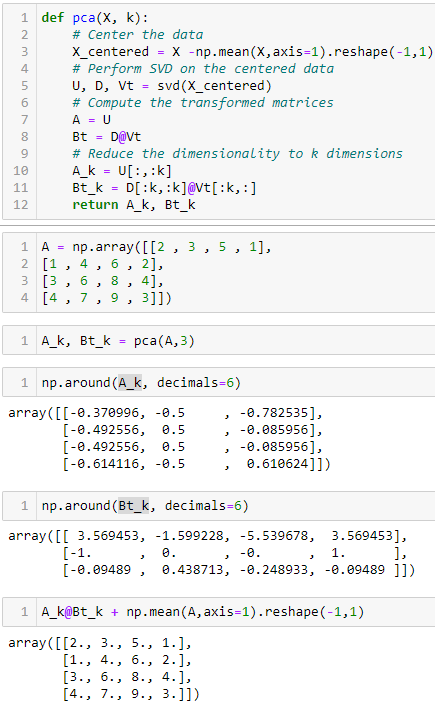
\includegraphics[scale=0.9]{implement_pca.png}
	\caption{Thử nghiệm thuật toán PCA trên PYTHON3}
	\label{fig:pca_example}
\end{figure}
\chapter{ MỘT SỐ ỨNG DỤNG CỦA SVD và PCA }

\section{Ứng dụng của SVD trong bài toán xấp xỉ hạng thấp tốt nhất của ma trận}

Về lí thuyết, khi làm việc với ma trận, ta cần nắm được toàn bộ những thông tin về ma trận đó. Tuy nhiên, trong thực tế có những ma trận cấp rất lớn với nhiều phần tử, lượng thông tin cần xử lí nhiều khiến ta rất khó khăn khi tiếp cận. Vấn đề đặt ra là, làm thế nào để ta cần loại bỏ, giảm tải bớt những thông tin, số liệu không cần thiết mà vẫn đảm bảo giữ lại những số liệu, những thông tin đặc trưng của ma trận, nhằm giúp cho công việc nghiên cứu được thuận tiện và đơn giản hơn. Nói cách khác, ta cần tìm một ma trận có hạng nhỏ hơn xấp xỉ với ma trận đã cho. Một trong những công cụ có thể giúp ta tìm được ma trận xấp xỉ đó chính là SVD. Trong chương này, chúng ta sẽ cùng tìm hiểu về ứng dụng của SVD trong bài toán xấp xỉ hạng thấp tốt nhất của ma trận. 

Cho $\mathbf{A}$ là một ma trận cấp $m \times n$ bất kì, $\operatorname{rank}(\mathbf{A})=r$. Giả sử $\mathbf{A}$ có phân tích SVD dạng khai triển là

$$
\mathbf{A}=\sum_{i=1}^{r} \sigma_{i} \mathbf{u}_{i} \mathbf{v}_{i}^{T}
$$

Với mỗi $k \in\{1,2, \ldots, r\}$, dặt

$$
\mathbf{A}_{k}=\sum_{i=1}^{k} \sigma_{i} \mathbf{u}_{i} \mathbf{v}_{i}^{T}
$$

Khi đó, $\operatorname{rank}\left(\mathbf{A}_{k}\right)=k$. Hơn nữa, $\mathbf{A}_{k}$ chính là ma trận xấp xỉ tốt nhất có hạng bằng $k$ của $\mathbf{A}$ theo cả hai chuẩn là chuẩn Frobenius và chuẩn 2. Ta có hai định lí quan trọng sau

\begin{dl}{Định lí Eckart- Young, 1936}  \label{eckart}

Với mọi ma trận $\mathbf{B}$ cỡ $m \times n$ và $\operatorname{rank}(\mathbf{B}) \leqslant k$, ta có

$$
\|\mathbf{A}-\mathbf{B}\|_{F} \geqslant\left\|\mathbf{A}-\mathbf{A}_{k}\right\|_{F} .
$$
\end{dl}
Để chứng minh Định lý Eckart- Young, ta cần Bổ đề sau

\begin{bd} \label{bode} Giả sử $\mathbf{A}$ là một ma trận cấp $m \times n$ bất kì, $\operatorname{rank}(\mathbf{A})=r, \mathbf{A}$ có phân tích SVD dạng khai triển là

$$
\mathbf{A}=\sum_{i=1}^{r} \sigma_{i} \mathbf{u}_{i} \mathbf{v}_{i}^{T}
$$

Khi đó với vector $\mathbf{x} \in \mathbb{R}^{n}$ bất kì và $1 \leqslant k \leqslant r$, ta có

$$
\|\mathbf{A} \mathbf{x}\|_{F}^{2} \leqslant \sigma_{k}^{2}\|\mathbf{x}\|_{F}^{2}+\sum_{i=1}^{k} \sigma_{i}^{2}\left(\mathbf{v}_{i}^{T} \mathbf{x}\right)^{2}-\sigma_{k}^{2} \sum_{i=1}^{k}\left(\mathbf{v}_{i}^{T} \mathbf{x}\right)^{2} .
$$
\end{bd}
\begin{proof}
Theo phân tích SVD dạng khai triển của $\mathbf{A}$ ta có

$$
\mathbf{A} \mathbf{x}=\sum_{i=1}^{r} \sigma_{i} \mathbf{u}_{i} \mathcal{V}_{i}^{T} \mathbf{x}=\sum_{i=1}^{r} \sigma_{i} \mathbf{u}_{i}\left(\mathcal{V}_{i}^{T} \mathbf{x}\right)=\sum_{i=1}^{r} \sigma_{i}\left(\mathcal{V}_{i}^{T} \mathbf{x}\right) \mathbf{u}_{i}
$$

Do $\left(\mathbf{u}_{1} \cdot \mathbf{u}_{2}, \ldots, \mathbf{u}_{m}\right)$ là cơ sở trực chuẩn trong $\mathbb{R}^{m}$ và $\sigma_{1} \geqslant \sigma_{2} \cdots \geqslant \sigma_{r}$ nên

$$
\|\mathbf{A} \mathbf{x}\|_{F}^{2}=\sum_{i=1}^{r} \sigma_{i}^{2}\left(\mathcal{V}_{i}^{T} \mathbf{x}\right)^{2} \leqslant \sum_{i=1}^{k} \sigma_{i}^{2}\left(\mathcal{V}_{i}^{T} \mathbf{x}\right)^{2}+\sigma_{k}^{2} \sum_{i=k+1}^{r}\left(\mathcal{V}_{i}^{T} \mathbf{x}\right)^{2} .
$$

Mặt khác

$\sigma_{k}^{2} \sum_{i=1}^{k}\left(\mathcal{V}_{i}^{T} \mathbf{x}\right)^{2}+\sigma_{k}^{2} \sum_{i=k+1}^{r}\left(\mathcal{V}_{i}^{T} \mathbf{x}\right)^{2}=\sigma_{k}^{2} \sum_{i=1}^{r}\left(\mathcal{V}_{i}^{T} \mathbf{x}\right)^{2} \leqslant \sigma_{k}^{2} \sum_{i=1}^{n}\left(\mathcal{V}_{i}^{T} \mathbf{x}\right)^{2}=\sigma_{k}^{2}\left\|\mathbf{V}^{T} \mathbf{x}\right\|_{F}^{2}=\sigma_{k}^{2}\|\mathbf{x}\|_{F}^{2}$

Do đó,

$$
\sigma_{k}^{2} \sum_{i=k+1}^{r}\left(\mathcal{V}_{i}^{T} \mathbf{x}\right)^{2} \leqslant \sigma_{k}^{2}\|\mathbf{x}\|_{F}^{2}-\sigma_{k}^{2} \sum_{i=1}^{k}\left(\mathcal{V}_{i}^{T} \mathbf{x}\right)^{2}
$$

Vậy

$$
\|\mathbf{A} \mathbf{x}\|_{F}^{2} \leqslant \sigma_{k}^{2}\|\mathbf{x}\|_{F}^{2}+\sum_{i=1}^{k} \sigma_{i}^{2}\left(\mathcal{V}_{i}^{T} \mathbf{x}\right)^{2}-\sigma_{k}^{2} \sum_{i=1}^{k}\left(\mathcal{V}_{i}^{T} \mathbf{x}\right)^{2}
$$
\end{proof}
Tiếp theo, chúng ta sẽ chứng minh Định lý Eckart-Young.
\begin{proof}
Định lý Eckart-Young. Giả sử ma trận $\mathbf{B}$ có khai triển SVD dạng

$$
\mathbf{B}=\sum_{i=1}^{k} \mathbf{x}_{i} \mathbf{y}_{i}^{T}
$$

trong đó $\left(\mathbf{x}_{1}, \mathbf{x}_{2}, \ldots, \mathbf{x}_{m}\right)$ là hệ trực giao, $\left(\mathbf{y}_{1}, \mathbf{y}_{2}, \ldots, \mathbf{y}_{n}\right)$ là hệ trực chuẩn. Ta có $\|\mathbf{A}-\mathbf{B}\|_{F}^{2}=\operatorname{Tr}\left((\mathbf{A}-\mathbf{B})\left(\mathbf{A}-\mathbf{B}^{T}\right)\right)=\operatorname{Tr}\left(\mathbf{A} \mathbf{A}^{T}-\mathbf{A} \mathbf{B}^{T}-\mathbf{B A}^{T}+\mathbf{B B}^{T}\right)$. Mặt khác

$$
\begin{aligned}
	\mathbf{B} \mathbf{B}^{T} & -\mathbf{A B}^{T}-\mathbf{B} \mathbf{A}^{T}=\left(\sum_{i=1}^{k} \mathbf{x}_{i} \mathbf{y}_{i}^{T}\right)\left(\sum_{i=1}^{k} \mathbf{y}_{i} \mathbf{x}_{i}^{T}\right)-A \sum_{i=1}^{k} \mathbf{y}_{i} \mathbf{x}_{i}^{T}-\left(\sum_{i=1}^{k} \mathbf{x}_{i} \mathbf{y}_{i}^{T}\right) \mathbf{A}^{T} \\
	& =\sum_{i=1}^{k} \mathbf{x}_{i} \mathbf{x}_{i}^{T}-\sum_{i=1}^{k} \mathbf{x}_{i} \mathbf{y}_{i}^{T} \mathbf{A}^{T}-\sum_{i=1}^{k} \mathbf{A}_{i} \mathbf{x}_{i}^{T}+\sum_{i=1}^{k} \mathbf{A}_{i} \mathbf{y}_{i}^{T} \mathbf{A}_{T}-\sum_{i=1}^{k} \mathbf{A}_{i} \mathbf{y}_{i}^{T} \mathbf{A}^{T} \\
	& =\sum_{i=1}^{k} \mathbf{x}_{i}\left(\mathbf{x}_{i}^{T}-\mathbf{y}_{i}^{T} \mathbf{A}^{T}\right)-\sum_{i=1}^{k} \mathbf{A} \mathbf{y}_{i}\left(\mathbf{x}_{i}^{T}-\mathbf{y}_{i}^{T} \mathbf{A}^{T}\right)-\sum_{i=1}^{k} \mathbf{A} \mathbf{y}_{i} \mathbf{y}_{i}^{T} \mathbf{A}^{T} \\
	& =\sum_{i=1}^{k}\left(\mathbf{x}_{i}-\mathbf{A} \mathbf{y}_{i}\right)\left(\mathbf{x}_{i}^{T}-\mathbf{y}_{i}^{T} \mathbf{A}^{T}\right)-\sum_{i=1}^{k} \mathbf{A} \mathbf{y}_{i} \mathbf{y}_{i}^{T} A^{T} \\
	& =\sum_{i=1}^{k}\left(\mathbf{x}_{i}-\mathbf{A} \mathbf{y}_{i}\right)\left(\mathbf{x}_{i}-\mathbf{y}_{i} \mathbf{A}\right)^{T}-\sum_{i=1}^{k}\left(\mathbf{A y}_{i}\right)\left(\mathbf{a y}_{i}\right)^{T} .
\end{aligned}
$$

Vì

$$
\left.\sum_{i=1}^{k} \operatorname{Tr}\left(\left(\mathbf{x}_{i}-\mathbf{A y}_{i}\right)\left(\mathbf{x}_{i}-\mathbf{y}_{i} \mathbf{A}\right)^{T}\right)\right)=\sum_{i=1}^{k}\left\|\mathbf{x}_{i}-\mathbf{A y}_{i}\right\|_{F}^{2} \geqslant 0
$$

nên suy ra

\begin{equation} \label{eq411}
\begin{aligned}
	\|\mathbf{A}-\mathbf{B}\|_{F}^{2} & =\operatorname{Tr}\left(\mathbf{A} \mathbf{A}^{T}\right)+\sum_{i=1}^{k} \operatorname{Tr}\left(\left(\mathbf{x}_{i}-\mathbf{A} \mathbf{y}_{i}\right)\left(\mathbf{x}_{i}-\mathbf{y}_{i} \mathbf{A}\right)^{T}\right)-\sum_{i=1}^{k}\left\|\mathbf{A y}_{i}\right\|_{F}^{2} \\
	& \geqslant \operatorname{Tr}\left(\mathbf{A} \mathbf{A}^{T}\right)-\sum_{i=1}^{k}\left\|\mathbf{A y}_{i}\right\|_{F}^{2} .
\end{aligned}
\end{equation}

Tiếp theo, ta đánh giá số hạng $\sum_{i=1}^{k}\left\|\mathbf{A y}_{i}\right\|_{F}^{2}$ trong bất đẳng thức \ref{eq411}. Theo Bổ đề \ref{bode} ta có

$$
\left\|\mathbf{A y}_{i}\right\|_{F}^{2} \leqslant \sigma_{k}^{2}+\sum_{i=1}^{k} \sigma_{i}^{2}\left(\mathcal{V}_{i}^{T} \mathbf{y}_{i}\right)^{2}-\sigma_{k}^{2} \sum_{i=1}^{k}\left(\mathcal{V}_{\mathcal{V}}^{T} \mathbf{y}_{i}\right)^{2} \text {. }
$$

Lấy tổng theo chỉ số $j$ ta có bất đẳng thức

$$
\begin{aligned}
	\sum_{j=1}^{k}\left\|\mathbf{A y}_{j}\right\|^{2} & \leqslant k \sigma_{k}^{2}+\sum_{j=1}^{k}\left[\sum_{i=1}^{k} \sigma_{i}^{2}\left(\mathcal{V}_{i}^{T} \mathbf{y}_{j}\right)^{2}-\sigma_{k}^{2} \sum_{i=1}^{k}\left(\mathcal{V}_{i}^{T} \mathbf{y}_{j}\right)^{2}\right] \\
	& =k \sigma_{k}^{2}+\sum_{j=1}^{k}\left[\sum_{i=1}^{k}\left(\sigma_{i}^{2}-\sigma_{k}^{2}\right)\left(\mathcal{V}_{i}^{T} \mathbf{y}_{j}\right)^{2}\right] \\
	& =\sum_{i=1}^{k}\left[\sigma_{k}^{2}+\sum_{j=1}^{k}\left(\sigma_{i}^{2}-\sigma_{k}^{2}\right)\left(\mathcal{V}_{i}^{T} \mathbf{y}_{j}\right)^{2}\right] \\
	& =\sum_{i=1}^{k}\left[\sigma_{k}^{2}+\left(\sigma_{i}^{2}-\sigma_{k}^{2}\right) \sum_{j=1}^{k}\left(v_{i}^{T} y_{j}\right)^{2}\right] .
\end{aligned}
$$

Mặt khác,

$$
\sum_{j=1}^{k}\left(\mathcal{V}_{i}^{T} \mathbf{y}_{j}\right)^{2} \leqslant \sum_{j=1}^{n}\left(\mathcal{V}_{i}^{T} \mathbf{y}_{j}\right)^{2}=\left\|\mathcal{V}_{i}^{T} \mathbf{Y}\right\|_{F}^{2}=\left\|\mathcal{V}_{i}^{T}\right\|_{F}^{2}=1
$$

với $\mathbf{Y}$ là ma trận trực giao có các cột là các vector $\mathbf{y}_{1}, \mathbf{y}_{2}, \ldots, \mathbf{y}_{n}$. Do đó

$$
\sum_{j=1}^{k}\left\|\mathbf{A y}_{j}\right\|_{F}^{2} \leqslant \sum_{i=1}^{k} \sigma_{k}^{2}
$$

Thay vào bất đẳng thức \ref{eq411} ta được

$$
\|\mathbf{A}-\mathbf{B}\|_{F}^{2} \geqslant \operatorname{Tr}\left(\mathbf{A} \mathbf{A}^{T}\right)-\sum_{i=1}^{k}\left\|\mathbf{A} \mathbf{y}_{i}\right\|_{F}^{2} \geqslant\|\mathbf{A}\|_{F}^{2}-\sum_{i=1}^{k} \sigma_{i}^{2} .
$$

Khi $\mathbf{B}=\mathbf{A}_{k}=\sum_{i=1}^{k} \sigma_{i} \mathbf{u}_{i} \mathcal{V}_{i}^{T}$, ta có

$$
\mathbf{A}-\mathbf{A}_{k}=\sum_{i=k+1}^{r} \sigma_{i} \mathbf{u}_{i} \mathcal{V}_{i}^{T}
$$

Từ đó suy ra

$$
\left\|\mathbf{A}-\mathbf{A}_{k}\right\|_{F}^{2}=\sum_{i=k+1}^{r} \sigma_{i}^{2}=\sum_{i=1}^{r} \sigma_{i}^{2}-\sum_{i=1}^{k} \sigma_{i}^{2}=\|A\|_{F}^{2}-\sum_{i=1}^{k} \sigma_{i}^{2} .
$$

Điều này chứng tỏ $\mathbf{A}_{k}$ chính là xấp xỉ hạng $k$ tốt nhất của ma trận $\mathbf{A}$ theo chuẩn Frobenius.
\end{proof}
Bên cạnh đó ta có nhận xét quan trọng về sai số do xấp xỉ một ma trận $\mathbf{A}$ có hạng $r$ bởi $mathbf{A}_{k}$ với $k < r$ phần tử như sau:

$$
	\label{eqn:26_17}
	\frac{\|\mathbf{A} - \mathbf{A}_k\|_F^2}{\|\mathbf{A}\|_F^2} = {\frac{\sum_{i=k+1}^{r} \sigma_{i}^{2}}{\sum_{i=1}^{r} \sigma_{i}^{2}}}
$$

Ở đây, {lượng thông tin} được định nghĩa
là tổng bình phương của giá trị suy biến. Ví dụ, nếu muốn giữ lại ít nhất
90\% lượng thông tin trong $\mathbf{A}$, trước hết ta tính $\sum_{j = 1}^r
\sigma_j^2$, sau đó chọn $k$ là số nhỏ nhất sao cho
$$
	\frac{\sum_{i = 1}^k \sigma_i^2}{\sum_{j = 1}^r \sigma_j^2} \geq 0.9
$$

\begin{dl}

Giả sử $\mathbf{A}$ là ma trận cỡ $m \times n$ bất kì, với $\operatorname{rank}(A)=r$ và $\mathbf{A}$ có khai triển kì dị SVD là

$$
\mathbf{A}=\sum_{i=1}^{r} \sigma_{i} \mathbf{u}_{i} \mathcal{V}_{i}^{T}
$$

Khi đó, với mọi ma trận $\mathbf{B}$ có cỡ $m \times n$ bất kì và $\operatorname{rank}(\mathbf{B}) \leqslant k$, ta có

$$
\|\mathbf{A}-\mathbf{B}\|_{2} \geqslant \sigma_{k+1}
$$

Dấu " =" xảy ra khi $\mathbf{B}=\mathbf{A}_{k}=\sum_{i=1}^{k} \sigma_{i} \mathbf{u}_{i} \mathcal{V}_{i}^{T}$.
\end{dl}

\begin{proof}
Giả sử tồn tại ma trận $\mathbf{B}$ có $\operatorname{rank}(\mathbf{B}) \leqslant k$ và $\|\mathbf{A}-\mathbf{B}\|_{2}<\sigma_{k+1}$. Vì $\operatorname{rank}(\mathbf{B}) \leqslant k$ nên tồn tại một không gian con $\mathbf{W}$ cỡ $r-k$ sao cho với mọi $\mathbf{w} \in \mathbf{W}$ thì $\mathrm{Bw}=0$.
Do đó với mọi $\mathbf{w} \in \mathbf{W}$ thì $\mathbf{A} \mathbf{w}=(\mathbf{A}-\mathbf{B}) \mathbf{w}$ và
$$
\|\mathbf{A} \mathbf{w}\|_{2}=\|(\mathbf{A}-\mathbf{B}) \mathbf{w}\|_{2} \leqslant\|\mathbf{A}-\mathbf{B}\|_{2}\|\mathbf{w}\|_{2}<\sigma_{k+1}\|\mathbf{w}\|_{2} .
$$

Vì vậy W là không gian con cỡ $r-k$ sao cho
$$
\|\mathbf{A}\|_{2}<\sigma_{k+1}\|\mathbf{w}\|_{2}
$$

Mặt khác, tồn tại một không gian con $\mathbf{U}$ có chiều là $k+1$ được xây dựng từ $k+1$ giá trị kì dị đầu tiên của ma trận $\mathbf{A}$ sao cho
$$
\|\mathbf{A} \mathbf{u}\| \geqslant \sigma_{k+1}\|\mathbf{u}\|_{2}, \quad \forall \mathbf{u} \in \mathbf{U}
$$

Khi đó $\operatorname{dim}(\mathbf{U}+\mathbf{W})=(r-k)+(k+1)=r+1>r$. Do đó tồn tại $\mathcal{V} \neq \mathbf{0}$ và $\mathcal{V} \in \mathbf{U} \cap \mathbf{W}$. Suy ra $\|\mathbf{A} \mathcal{V}\|_{2}<\sigma_{k+1}\|\mathcal{V}\|_{2}$ và $\|\mathbf{A} \mathcal{V}\| \geqslant \sigma_{k+1}\|\mathcal{V}\|_{2}$. Điều này không thể xảy ra. Vì vậy giả thiết phản chứng ban đầu là sai.

Vậy với mọi ma trận $\mathbf{B}$ cỡ $m \times n$ bất kì có $\operatorname{rank}(\mathbf{B}) \leqslant k$ thì $\|\mathbf{A}-\mathbf{B}\|_{2} \geqslant \sigma_{k+1}$.

Khi $\mathbf{B}=\mathbf{A}_{k}$ thì $\left\|\mathbf{A}-\mathbf{A}_{k}\right\|_{2}=\sigma_{k+1}$. Điều này chứng tỏ $\mathbf{A}_{k}$ chính là xấp xỉ hạng $k$ tốt nhất của $\mathbf{A}$ theo chuẩn 2 . 
\end{proof}

\section{Phân tích SVD trong xử lí ảnh}

Như đã nói, phân tích SVD là dạng phân tích có rất nhiều ứng dụng trong lý thuyết và thực tiễn. Một trong những ứng dụng ấn tượng nhất chính là sử dụng SVD trong hiệu chỉnh hình ảnh kĩ thuật số. Nhờ đó hình ảnh được truyền đi một cách hiệu quả bằng vệ tinh, internet, ...

Ý tưởng cơ sở của việc hiệu chỉnh ảnh là làm giảm số lượng thông tin truyền đi mà không làm mất đi những thông tin thực chất. Trong một bức ảnh kĩ thuật số, mỗi điểm ảnh được thể hiện bởi ba giá trị màu: xanh (blue), lục (green), đỏ (red) với các trị số từ 0 đến 255. Như vậy, với một hình ảnh chỉ với độ lớn là $130 \times 130$ pixels thì chúng ta phải lưu trữ 3 ma trận (thể hiện màu sắc của các điểm) có cùng độ lớn là $130 \times 130$, tức là phải lưu trữ 50700 số. Tuy nhiên, trong thực tế, khi truyền hay lưu trữ thông tin ảnh, ta có thể không cần những hình ảnh, hoặc một số phần của hình ảnh có độ nét quá lớn. Sử dụng phân tích SVD, chúng ta có thể loại bỏ rất nhiều thông tin không cần thiết đó.

Ví dụ một hình ảnh $130 \times 130$ pixels được phân tích thành 3 ma trận $\mathbf{A}, \mathbf{B}, \mathbf{C}$ có cùng độ lớn $130 \times 130$. Giả sử $\mathbf{A}$ có phân tích SVD là

$$
\mathbf{A}=\sigma_{1} \mathbf{u}_{1} \mathcal{V}_{1}^{T}+\cdots+\sigma_{r} \mathbf{u}_{r} \mathcal{V}_{r}^{T}
$$

Theo như chứng minh ở Định lí \ref{eckart} với mỗi giá trị $k<r$ thì $A_{k}=\sigma_{1} \mathbf{u}_{1} \mathcal{V}_{1}^{T}+\cdots+$ $\sigma_{k} \mathbf{u}_{k} \mathcal{V}_{k}^{T}$ là xấp xỉ hạng $k$ tốt nhất của $\mathbf{A}$.

Ví dụ, $k=16$ thì ma trận $\mathbf{A}_{k}$ thể hiện các dữ liệu của $\mathbf{A}$ tương ứng với 16 giá trị kì dị đầu tiên. Như vậy, ta chỉ cần lưu trữ 16 giá trị kì dị, 16 vector $\mathbf{u}_{i}, 16z $ vector $\mathcal{V}_{i}$, tương đương với 4176 số. Tương tự như vậy với hai ma trận $\mathbf{B}$ và $\mathbf{C}$, số lượng các số phải lưu trữ là 12528 số. Rõ ràng phân tích SVD đã giúp giảm tải một lượng thông tin cần lưu trữ một cách đáng kể.

Trong  Python, ta có thể hiệu chỉnh độ nét của hình ảnh theo tham số $k$ tùy chọn. Ta xét ví dụ sau để đơn giản ta chỉ xét hình ảnh xám với kích cỡ $130 \times 130 \times1 $ như sau :

\begin{figure}[htp]
	\centering
	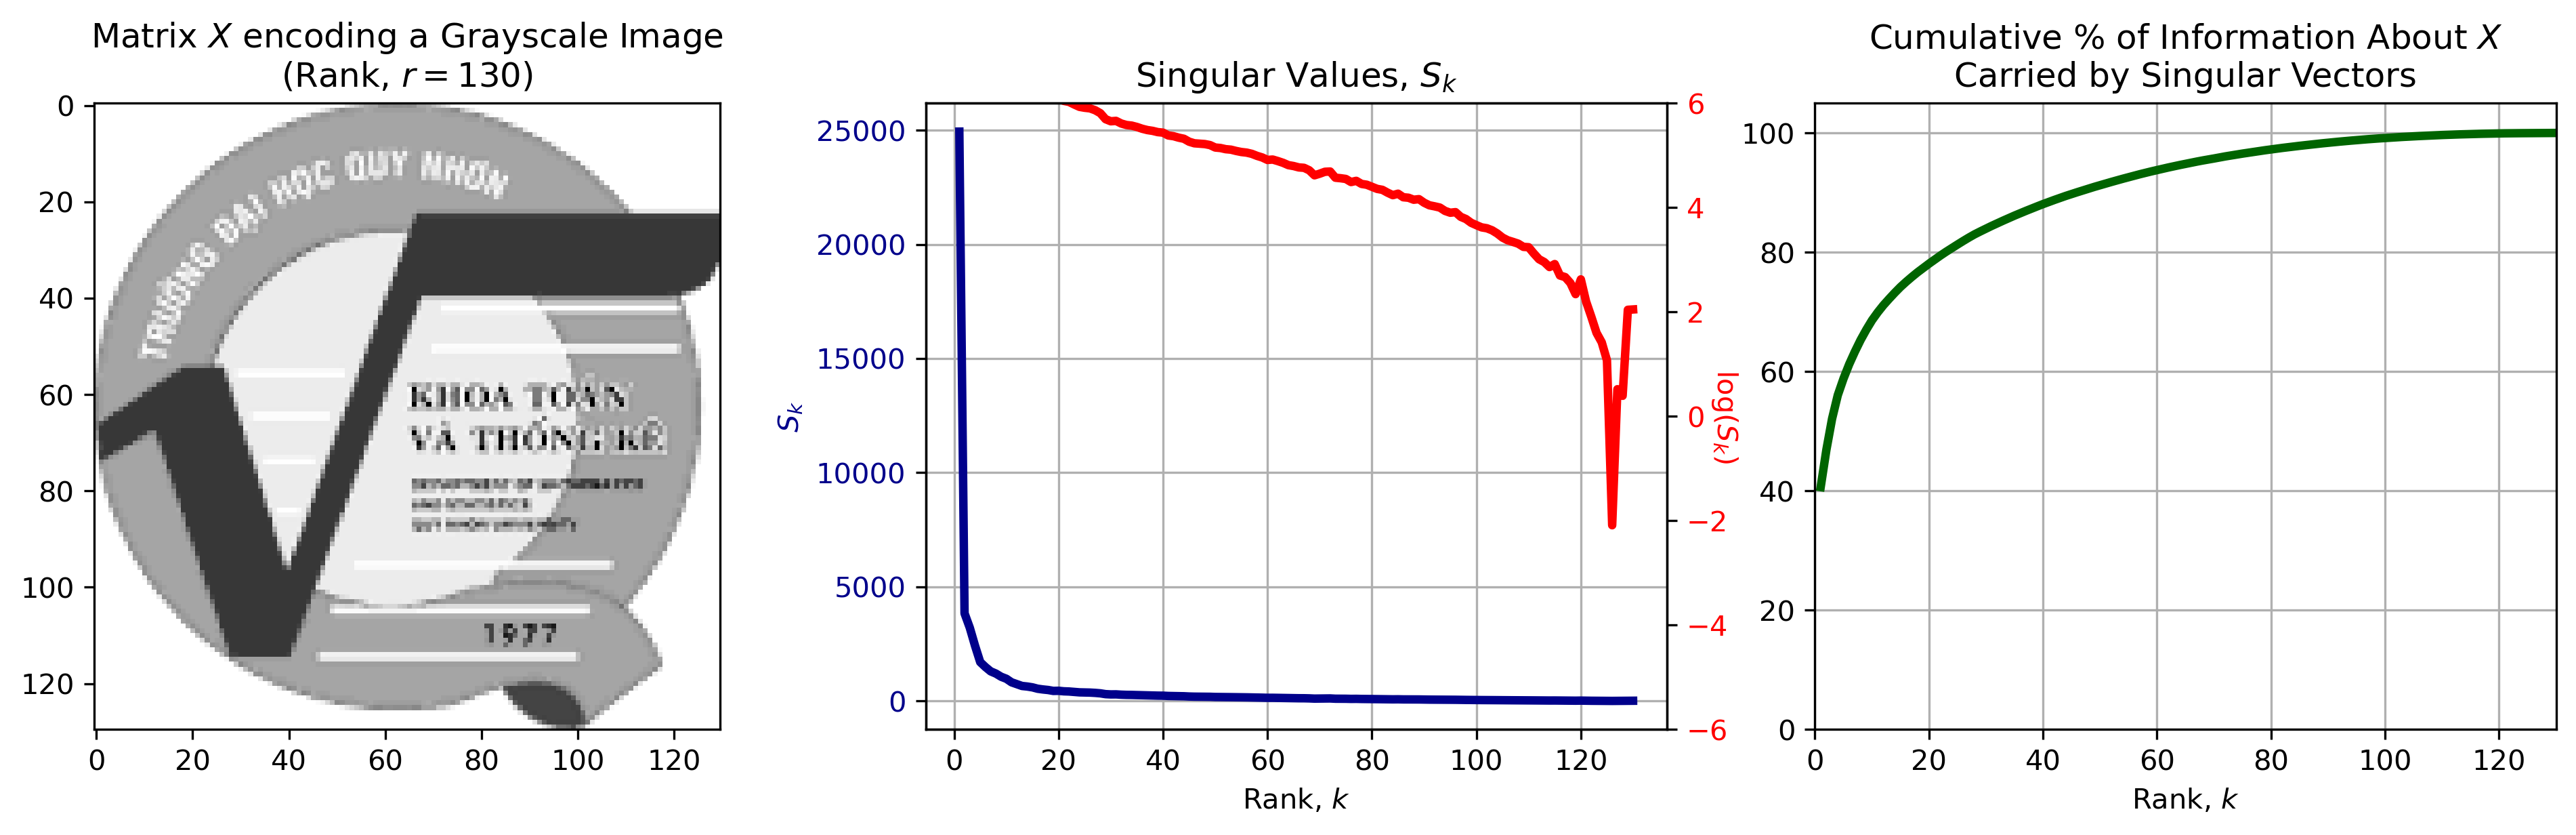
\includegraphics[scale=0.5]{image-singular-values.png}
	\caption{Tính quan trọng của các thành phần chính trong ma trận ảnh và mức độ giữ lại thông tin khi ta giảm số lượng các thành phần chính}
	\label{fig:svd_sigular}
\end{figure}

Đồ thị đầu tiên (bên trái) hiển thị ma trận ảnh gốc, được biểu diễn bằng các giá trị màu xám. Ma trận này thể hiện hình ảnh ban đầu trước bất kỳ xử lý nào.Đồ thị thứ hai (ở giữa) biểu diễn các giá trị kì dị (singular values) của ma trận ảnh. Các giá trị kì dị thể hiện độ lớn của các thành phần chính trong ma trận. Đồ thị hiển thị hai đường: một đường cho các giá trị kì dị ban đầu và một đường cho các giá trị kì dụ được chuyển đổi sang đơn vị logarit (logarithmic scale). Biểu đồ này cho ta cái nhìn tổng quan về độ quan trọng của các thành phần chính trong ma trận ảnh.Đồ thị cuối cùng (bên phải) biểu diễn tổng hợp thông tin tích lũy bằng cách sử dụng các giá trị kì dị. Nó cho thấy phần trăm thông tin được giữ lại (tích lũy) khi ta giữ lại một số lượng gia tăng các thành phần chính. Đồ thị này giúp ta quyết định xem ta có thể giảm số lượng thành phần chính mà không mất quá nhiều thông tin quan trọng.
Cụ thế hơn khi giảm chiều dữ liệu với $k = 4,16, 32 ,64.$. Ta thấy với việc sấp xỉ ma trận ban đầu bằng SVD với $ k=32 $ ta đã giảm được dung lương lưu trữ đi khoảng $50\%$ nhưng vẫn không làm giảm đi chất lượng hình ảnh quá nhiều.

Lưu ý: 
\begin{itemize}
	\item Compression là tỉ lệ dung lượng đã giảm được để lưu trữ hình ảnh nén.
	\item Info. Retained là phần thông tin từ ma trận gốc mà chúng ta vẫn giữ được sau khi nén.
\end{itemize}

\begin{figure}[htp]
	\centering
	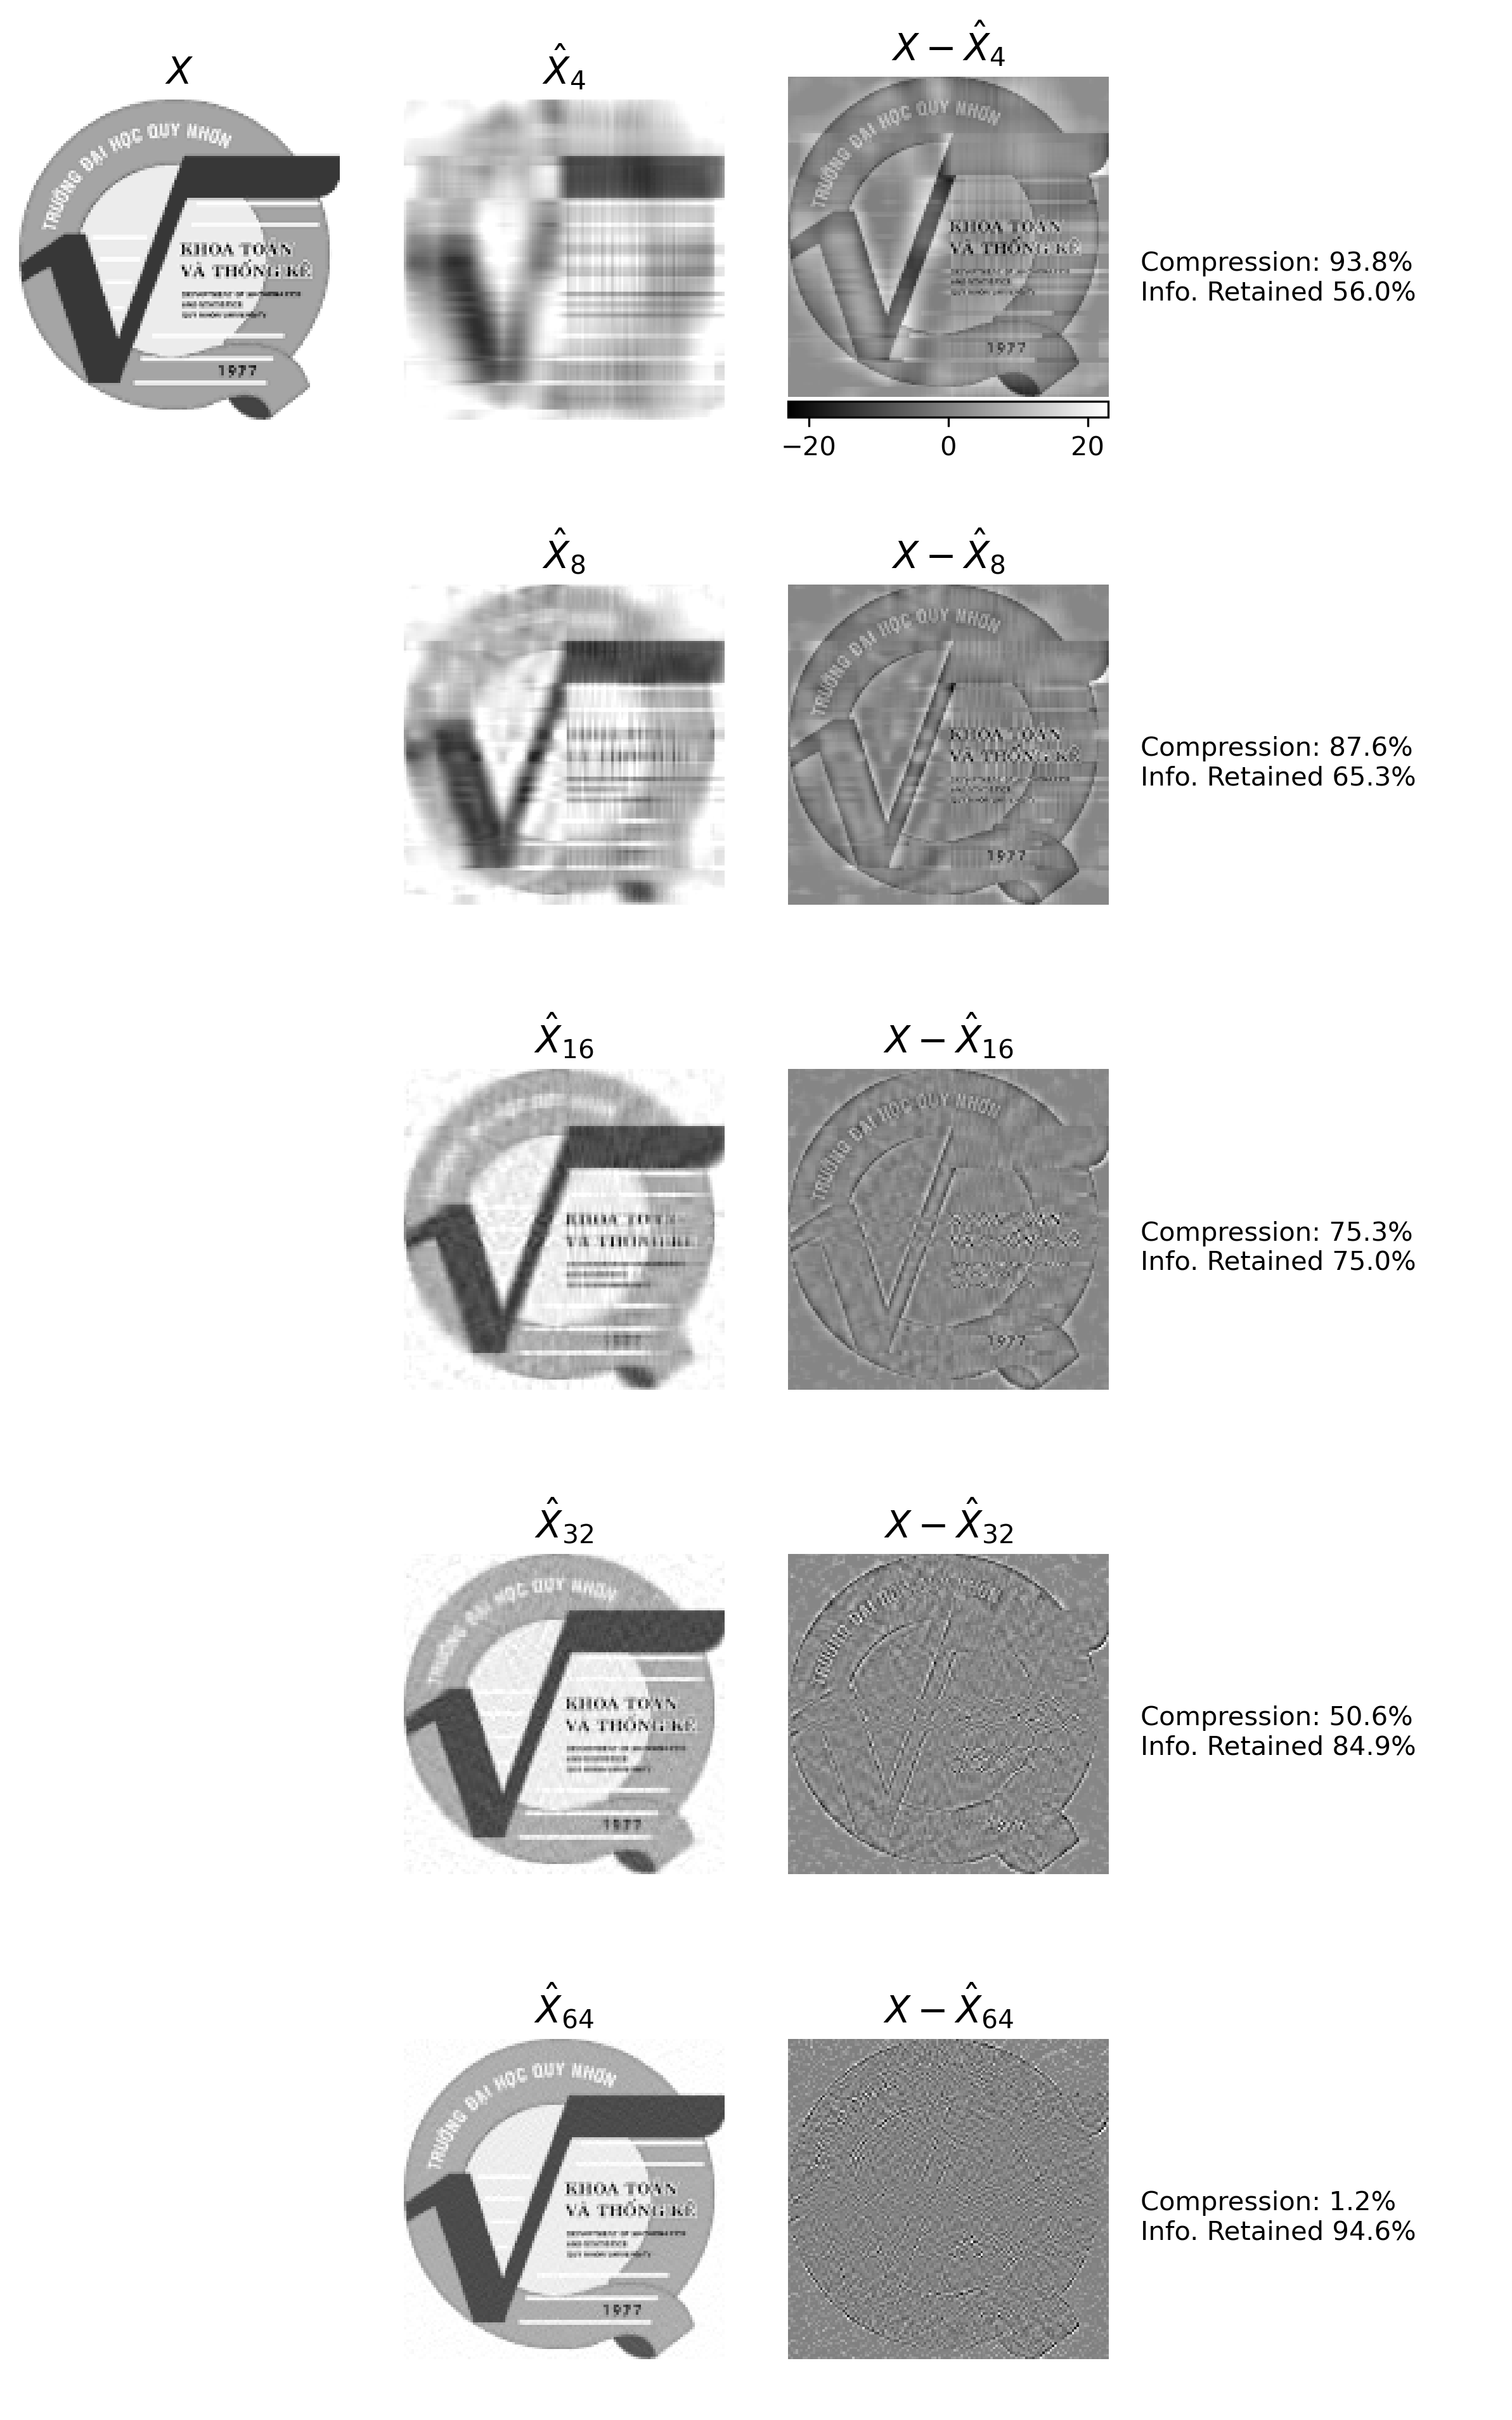
\includegraphics[scale=0.7]{svd_qnu.png}
	\caption{Ứng với từng $k$ ta quan sát được mức độ tối ưu trong việc lưu trữ thông tin cũng như là lượng thông tin được giữ lại.}
	\label{fig:svd_qnu}
\end{figure}
\newpage
\section{Eigenface và ứng dụng PCA trong nhận dạng khuôn mặt}
Phân tích thành phần chính (PCA - Principal Component Analysis) luôn được biết đến như là một phương pháp thống kê phổ biến dùng để giảm kích thước của dữ liệu trong khi vẫn giữ được những thông tin quan trọng nhất. PCA tìm ra các "thành phần chính" trong dữ liệu - những hướng mà dữ liệu biến đổi nhiều nhất, và dùng chúng để tái biểu diễn dữ liệu trong một không gian ít chiều hơn. Do đó, PCA đóng một vai trò quan trọng trong lĩnh vực nhận dạng khuôn mặt. Nhận dạng khuôn mặt là một bài toán phức tạp do sự đa dạng vô cùng lớn của các khuôn mặt. Mỗi khuôn mặt đều có những đặc điểm duy nhất và khác biệt như kích thước, hình dạng, màu sắc, cấu trúc, đặc điểm về giới tính, tuổi tác, v.v... PCA giúp chúng ta tìm ra những đặc điểm quan trọng nhất (hay còn gọi là "thành phần chính") của khuôn mặt, giúp tối ưu hóa quá trình nhận dạng và giảm bớt chi phí tính toán. Một trong những phương pháp thường được biết đến đó là Eigenface.

Eigenface là một phương pháp nhận dạng khuôn mặt dựa trên kỹ thuật phân tích thành phần chính (PCA). Thuật ngữ "Eigenface" xuất phát từ từ "eigen" trong tiếng Đức, có nghĩa là "đặc trưng" hoặc "riêng". Trong ngữ cảnh này, một Eigenface là một tập hợp các vector riêng, mà từ đó có thể tạo ra hầu hết các khuôn mặt khác nhau.

Phương pháp Eigenface giảm kích thước của dữ liệu hình ảnh khuôn mặt bằng cách chuyển đổi nó thành một tập hợp các thành phần chính. Những thành phần này, được gọi là Eigenfaces, đại diện cho các đặc điểm cơ bản của khuôn mặt, như hình dạng của mắt, mũi, miệng và vị trí tương đối của chúng. Mỗi khuôn mặt trong dữ liệu đều có thể được biểu diễn như một tổ hợp tuyến tính của những Eigenface này. Tôi sẽ thử nghiệm phương pháp Eigenface trên bộ dữ liệu LFW.

Bộ dữ liệu LFW (Labeled Faces in the Wild) là một bộ dữ liệu hình ảnh khuôn mặt phổ biến được sử dụng trong nghiên cứu nhận dạng khuôn mặt. Bộ dữ liệu này bao gồm hình ảnh của hàng trăm người nổi tiếng, với mỗi người được chụp dưới nhiều góc độ và biểu cảm khác nhau. Mỗi hình ảnh trong bộ dữ liệu là một ma trận hai chiều biểu thị giá trị cường độ điểm ảnh có thể hiểu như ma trận $50*37*1$. với 1288 hình. Và được chia thành 7 loại khác nhau ứng với 7 người nổi tiểng.

Khi áp dụng phương pháp Eigenface cho bộ dữ liệu LFW, ta sẽ tạo ra một "khuôn mặt trung bình" cùng với một tập hợp các "Eigenfaces". Sau đó, mỗi khuôn mặt trong bộ dữ liệu có thể được biểu diễn như một tổ hợp tuyến tính của các Eigenfaces, giúp cho việc nhận dạng khuôn mặt trở nên hiệu quả và chính xác hơn.

Đầu tiên ta sẽ làm "phẳng" ma trận đầu vào thành ma trận $(50*37,1288)$ với mỗi cột là một vector ứng với một khuôn mặt trong tập dữ liệu. Sau đó ta chia dữ liệu đầu vào thành tập huấn luyện và tập kiểm thử với tỉ lể lần lượt là 0.75 và 0.25. Ta nhận được 2 ma trận với kích cỡ là $(1850,966)$ và $(1850,322)$

%Sau đó ta đi tìm Eigenface cho mỗi khung mặt trên tập huấn luyện và ma trận biểu diễn dữ liệu gốc trên cơ sở của các thành phần chính($\mathbf{B}_k^T$) thông qua PCA.
Sau đó, ta đi tìm ma trận $\mathbf{A}_k$ chứa các Eigenfaces và ma trận biểu diễn dữ liệu gốc trên cơ sở của các thành phần chính $\mathbf{B}_k^T$ thông qua PCA.

PCA sẽ giúp chúng ta xác định các thành phần chính (hay còn gọi là Eigenfaces trong ngữ cảnh này) của tập dữ liệu hình ảnh khuôn mặt. Các thành phần này, được chứa trong ma trận $\mathbf{A}_k$, đại diện cho các hướng mà dữ liệu biến thiên nhiều nhất. Điều này giúp tạo ra một không gian mới, với các trục tương ứng với các thành phần chính, để biểu diễn dữ liệu.

Kế tiếp, chúng ta tính toán ma trận $\mathbf{B}_k^T$, mà mỗi cột của nó biểu diễn một hình ảnh khuôn mặt trong không gian của các thành phần chính. Mỗi hình ảnh khuôn mặt giờ đây được biểu diễn bằng một tổ hợp tuyến tính của các Eigenfaces, với hệ số tương ứng nằm trong $\mathbf{B}_k^T$.

Vì vậy, thông qua PCA, chúng ta có thể giảm đáng kể số lượng chiều dữ liệu mà vẫn giữ được phần lớn thông tin cần thiết từ tập dữ liệu hình ảnh khuôn mặt ban đầu. Với $k =150$ ta có thể xem kết quả sau khi được kết quả ảnh sau khi qua PCA Hình \ref{fig:eigenface}
\begin{figure}[htp]
	\centering
	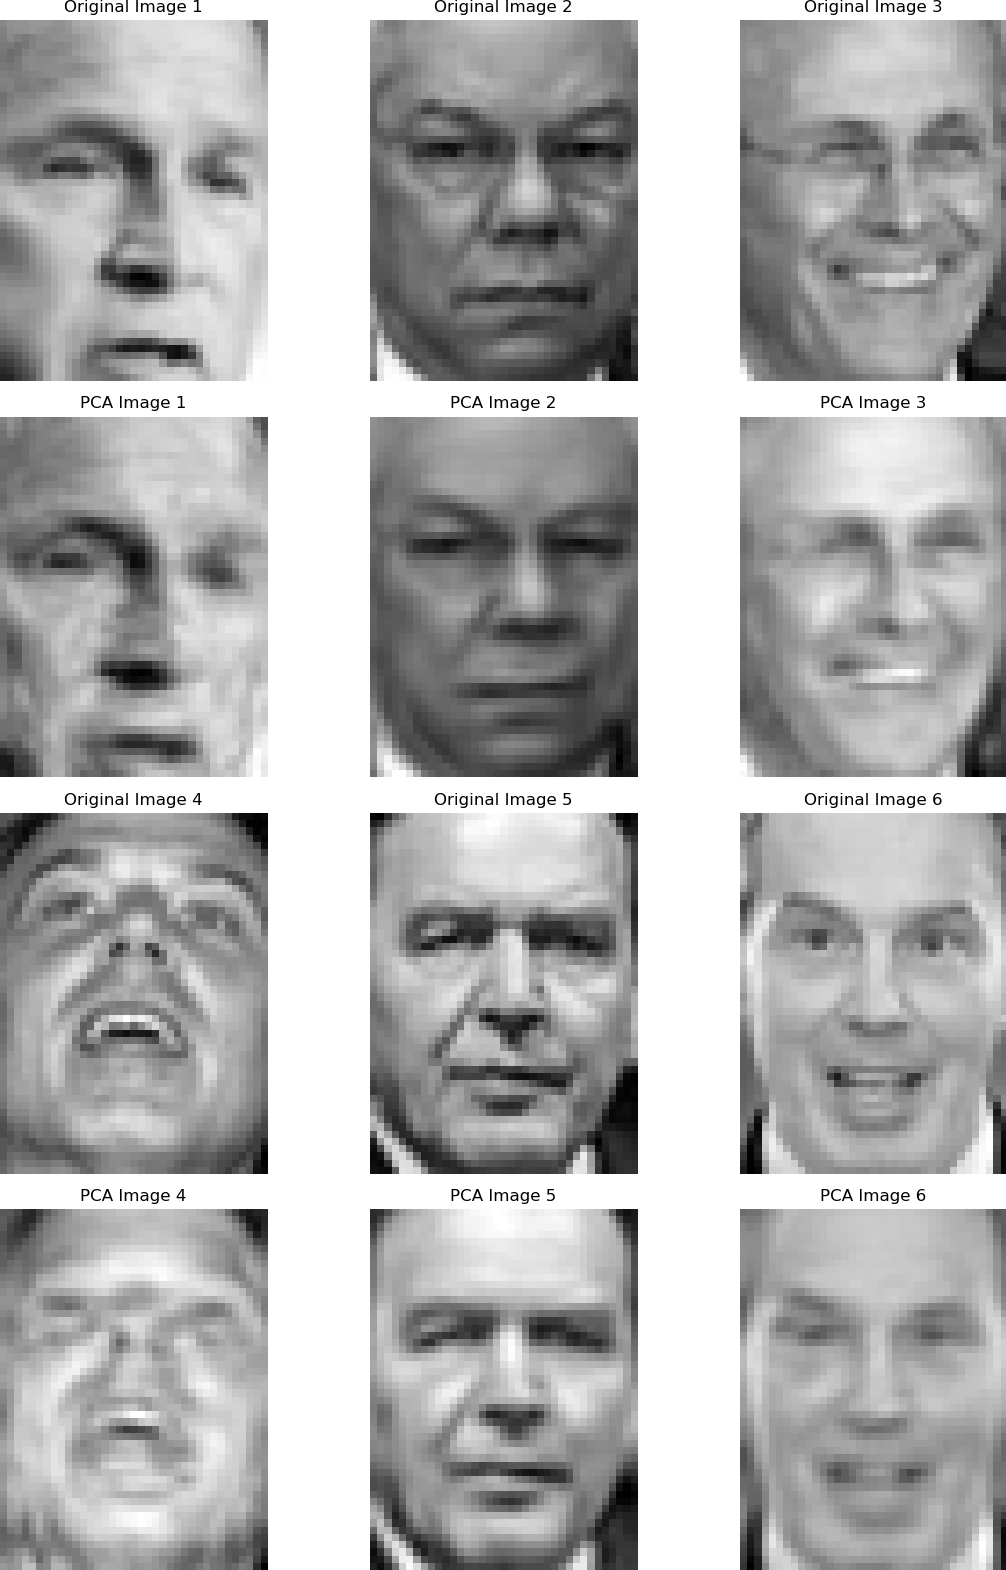
\includegraphics[scale=0.62]{eigenface.png}
	\caption{Hình ảnh ban đầu và hình ảnh sau khi được khôi phục qua PCA.}
	\label{fig:eigenface}
\end{figure}

Sau đó giảm chiều dữ liệu kiểm thử bằng cách chiếu nó qua ma trận $\mathbf{A}_k$ theo công thức \ref{chieu}.
Bây giờ ta có 966 điểm dữ liệu huấn liệu và 322 điểm dữ liệu kiểm thử. Liệu ta có thể phân biệt được các nét đặc trưng của mỗi khuông mặt chỉ thông qua các vector eigenface chỉ với 150 chiều thay và 1850 như ban đầu.
Để trả lời câu hỏi này ta sẽ huấn luyện một bộ phân lớp tương đối nổi tiếng và SVM(support Vector Machine).
hình \ref{fig:svm_result} và hình \ref{fig:headmap}  là kết quả sau khi thử nghiệm với bộ phân loại SVM. Ta thấy bộ phân loại có thể nhận dạng khuôn mặt tốt dựa trên vector eigenface với độ chính xác trùng bình là $80\%$. Hình \ref{fig:output} là kết quả suy luận của bộ phân loại trên tập kiểm thử.
\begin{figure}[htp]
	\centering
	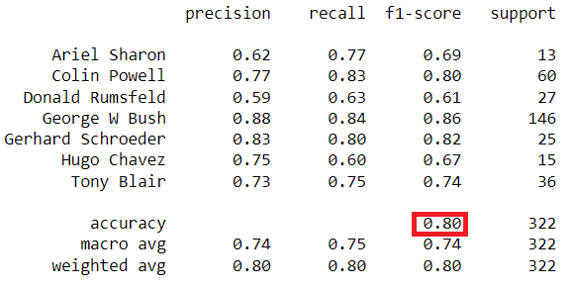
\includegraphics[scale=0.8]{result_svm.png}
	\caption{kết quả sau khi huận luyện bộ phân loại SVM.}
	\label{fig:svm_result}
\end{figure}
\begin{figure}[htp]
	\centering
	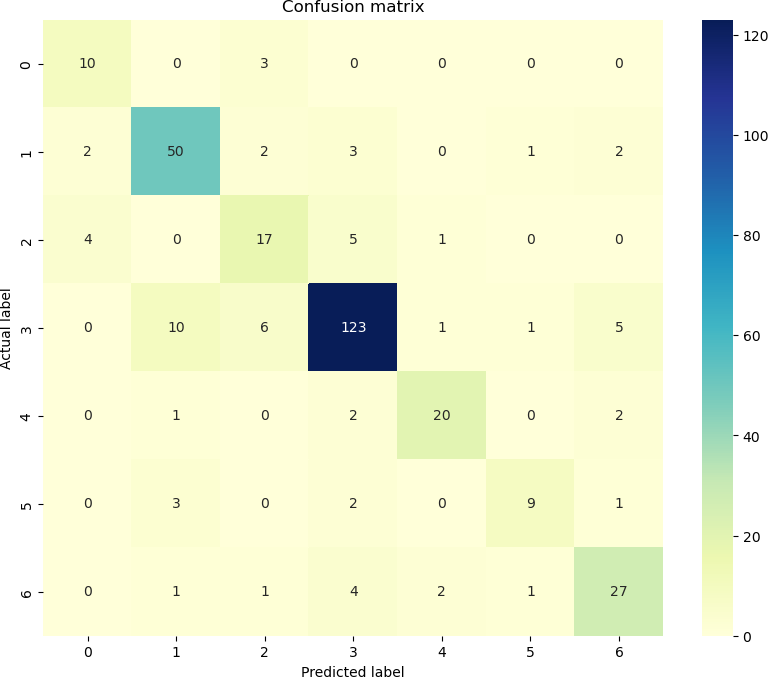
\includegraphics[scale=0.8]{heatmap.png}
	\caption{Ma trận lỗi(confusion matrix)}
	\label{fig:headmap}
\end{figure}

\begin{figure}[htp]
	\centering
	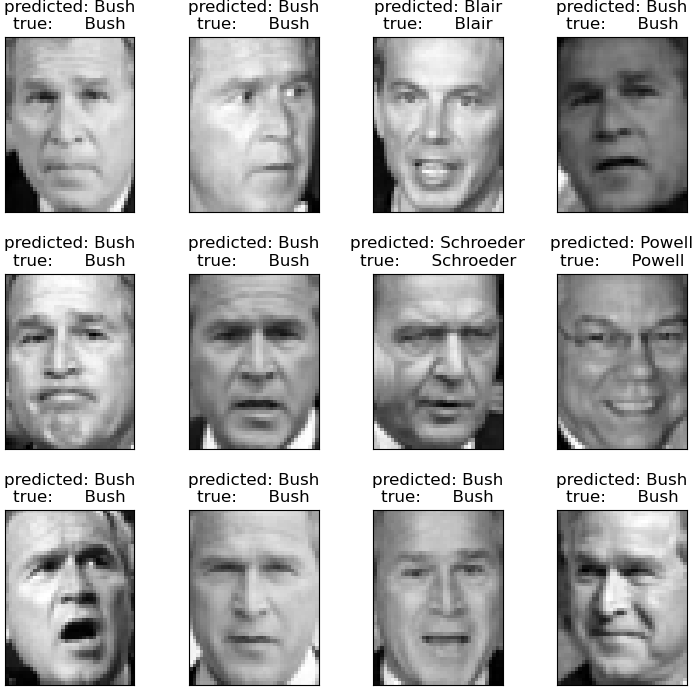
\includegraphics[scale=0.8]{predict_pca.png}
	\caption{kết quả suy luận của bộ phân loại trên tập kiểm thử}
	\label{fig:output}
\end{figure}
\chapter{Kết luận}
Qua quá trình thực hiện khóa luận, tôi đã có cơ hội tìm hiểu và nghiên cứu sâu về các khái niệm và kỹ thuật liên quan đến Phân tích giá trị kì dị (SVD) và Phân tích thành phần chính (PCA). Khóa luận đã đạt được những kết quả sau:
\begin{itemize}
	\item[1]Kiến thức chuẩn bị: Khóa luận đã trình bày một cách tổng quát về các kiến thức cơ bản về Ma trận, Vector riêng, Giá trị riêng, và Định lí phổ của ma trận đối xứng. Đồng thời, khóa luận cũng đã giới thiệu về các khái niệm cơ bản trong Xác xuất thống kê bao gồm Kỳ vọng, Phương sai và Ma trận hiệp phương sai.

\item[1]Phân tích giá trị kì dị (SVD): Khóa luận đã giới thiệu về khái niệm SVD, cách thức tính toán SVD của một ma trận, cũng như một số tính chất quan trọng của ma trận liên quan đến SVD.

\item[3]Phân tích thành phần chính (PCA): Khóa luận đã trình bày về khái niệm PCA, ý tưởng chính của PCA, cách thức tìm các thành phần chính của bài toán PCA thông qua SVD, tính duy nhất của nghiệm của PCA, và cũng đã giới thiệu về thuật toán tìm PCA của một ma trận.

\item[4]Một số ứng dụng của SVD và PCA: Khóa luận đã giới thiệu về một số ứng dụng thực tế của SVD và PCA, bao gồm việc sử dụng SVD trong bài toán xấp xỉ hạng thấp tốt nhất của ma trận, ứng dụng của SVD trong xử lý ảnh, và cách sử dụng PCA trong bài toán nhận dạng khuôn mặt thông qua phương pháp Eigenface.
\end{itemize}
Mặc dù khóa luận đã cố gắng trình bày một cách đầy đủ và chi tiết, nhưng không tránh khỏi những thiếu sót. Tôi rất mong nhận được những ý kiến đóng góp từ Quý Thầy, Cô và các bạn để có thể hoàn thiện hơn trong việc nghiên cứu và ứng dụng các kiến thức liên quan đến SVD và PCA trong tương lai.


\begin{thebibliography}{99}

\bibitem{thuan2003}
Nguyễn Duy Thuận, Phi Mạnh Ban, Nông Quốc Chinh,
\emph{Dại số tuyến tính},
Nhà xuất bản Đại học Sư phạm, (2003).

\bibitem{hieu2019}
Lê Thanh Hiếu,
\emph{Giáo trình đại số tuyến tính 1,2},
Giáo trình lưu hành nội bộ, (2019).

\bibitem{tien2018}
Vũ Hữu Tiệp,
\emph{Machine Learning cơ bản},
Nhà xuất bản Khoa học và Kỹ thuật, (2018).

\bibitem{hyvarinen2009}
Aapo Hyvärinen,
\emph{Principal component analysis},
Based on material from the book Natural Image Statistics to be published by Springer-Verlag in 2009.

\bibitem{meyer2000}
Carl D. Meyer,
\emph{Matrix analysis and applied linear algebra},
SIAM, Philadelphia 2000.


\bibitem{lay1994}
David C. Lay,
\emph{Linear algebra and its applications},
Addison-Wesley, Reading, MA, 1994.

\bibitem{eckart1936}
Eckart, C.; Young, G. (1936). "The approximation of one matrix by another of lower rank". Psychometrika. 1 (3): 211–8. doi:10.1007/BF02288367. S2CID 10163399.

\bibitem{harshman1970}
Harshman R. A.,
\emph{Foundations of Parafac procedure: Models and conditions for an "explanatory" multimodal factor analysis},
UCLA Working papers in Phonetics, 16, p.1-84, 1970.

\bibitem{good1969}
I. J. Good,
\emph{Some applications of the singular value decomposition of matrix},
Technometrics, 11, p. 823-831, 1969.


\bibitem{stewart1993}
Stewart G. W.,
\emph{On the early history of the singular value decomposition},
SIAM Review, 35, p. 551-566, 1993.

\bibitem{sgores2000}
Thomas S. Sgores,
\emph{Applied linear algebra and matrix analysis},
Springer, 2000.

\bibitem{website}
\url{https://tuanvanle.wordpress.com/2013/12/25/phuongphap-phan-tich-thanh-phan-chinh-principal-component-analysispca}
\url{https://en.wikipedia.org/wiki/Singular_value_decomposition#History}
	\end{thebibliography}
\end{document}




   
   
   
   
   
   
   
   
   
   